
\par
Najbardziej rozpoznawalne dwie przeglądarki Osirix i Horus, posiadają swoje nazwy od bogów egipskich.
Odpowiednio od Ozyrysa, boga śmierci i Horusa, boga nieba.
Dlatego postanowiłem nazwać swoja przeglądarkę w podobny sposób: Sokar.
\par
Sokar w mitologii egipskiej to bóstwo dokonujące przyjęcia i oczyszczenia zmarłego władcy oraz przenoszący go na swej barce do niebios, patron metalurgów, rzemieślników i tragarzy (nosicieli lektyk) oraz wszelkich przewoźników.

\section{Zakres implementacji}

\par
Po analizie możliwości przeglądarek plików DICOM dostępnych na rynku postanowiłem zaimplementować następujące komponenty w mojej przeglądarce:
\begin{itemize}
    \item Obsługa obrazów bez względu na ich modalność, ale z ograniczeniem do następujących interpretacji fotometrycznej:

          \begin{itemize}
              \item \dataword{MONOCHROME1}
              \item \dataword{MONOCHROME2}
              \item \dataword{RGB}
              \item \dataword{YBR}
          \end{itemize}

    \item Przesuwanie \fromEng{pan}

    \item Skalowaniu lub powiększenie poprzez decymacje i interpolacje liniowe.

    \item Rotacja i odbicia lustrzane

    \item Okienkowanie i pseudokolorowanie, zarówno w skali szarości jak i z użyciem wielo kolorowych palet.

    \item Obsługa serii obrazów jako całości
          \begin{itemize}
              \item przegląd obrazów w serii
              \item animacje
              \item wspólne okna w skali barwnej
          \end{itemize}
\end{itemize}


\section{Wieloplatformowość}
\par
Dla uzyskania wieloplatformowości kodu źródłowego zastosowano biblioteki: GDCM i Qt.
Przestrzegano standardu C++ w standardzie ISO/IEC 14882 z 2018, w skrócie C++17.
Zapewniono procedury kompilacji na wszystkie platformy poprzez użycia narzędzia CMake.


\section{Opis interfejsu graficznego użytkownika}

\par
Po uruchomieniu programu użytkownikowi ukazuje się jedno okno (rysunek \ref{sec:gui-window}), które zawiera 3 elementy: menu (obiekt klasy \qtclass{QMenuBar}), drzewa plików (obiekt klasy \sokarclass{FileTree}), obiekt zakładek z obrazami (obiekt klasy \sokarclass{DicomTabs}).
\par
Użytkownik może otworzyć plik DICOM na trzy sposoby: z menu na górze, z drzewem ze strukturą pików i poprzez przeciągnięcie.

\section{Projekt struktury obiektowej programu}
\sokarclassExplanations

\par
W tej sekcji wyjaśniona jest ogólna struktura programu, z pominięciem dokładnych opisów poszczególnych elementów.
Ich szczegółowy opis znajduje się w następnych sekcjach.
\par
Obiekt okna, klasy \sokarclass{MainWindow} posiada 3 elementy: menu (klasy \qtclass{QMenuBar}), drzewa plików (klasy \sokarclass{FileTree}), obiekt zakładek (klasy \sokarclass{DicomTabs}).
Zakładki obiektu zakładek są implementowane prze klasę \sokarclass{DicomView}.
Obiekt zakładki posiada abstrakcyjną kolekcję scen, implementowaną przez \sokarclass{DicomSceneSet}.
Kolekcja scen odpowiada za przechowywanie obrazów i scen, obiektów klasy \sokarclass{DicomScene}.
Sceny nie posiadają bezpośredniego dostępu do pliku, a jednie wskaźniki do odpowiednich miejsc w pamięci, gdzie obrazy są przechowywane.
Ogólny diagram klas znajduje się na rysunku \ref{fig:uml-global-sturcture}.

\begin{figure}[!htbp]
    \centering
    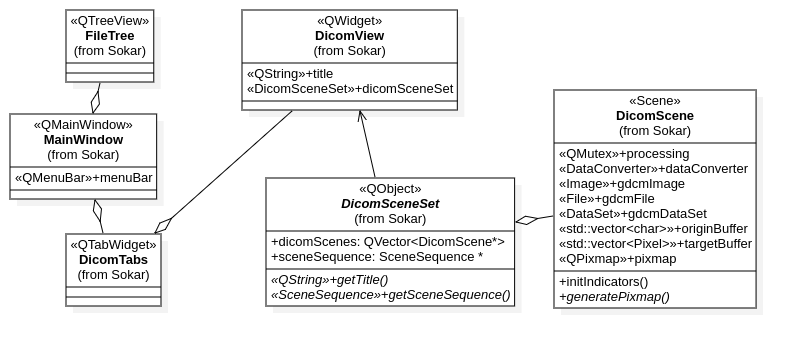
\includegraphics[width=\textwidth]{img/uml/global-sturcture.png}
    \caption{Diagram klas UML globalnej struktury programu.}
    \label{fig:uml-global-sturcture}
\end{figure}


\section{Struktury danych}

\subsection{Konwertowanie danych z znacznikach}

\par
Każdy plik \DICOM posiada zbiór elementów danych.
Zapisane elementy danych należy przekonwertować na obiekty danych odpowiadające potrzebom programu.
%https://sjp.pl/przekonwertowa%C4%87
Dlatego został zaimplementowany obiekt klasy \sokarclass{DataConverter} zajmujący się konwersją danych z pliku \DICOM na dane w formacie odpowiadającym programowi.

\par
Obiekt konwertera jest tworzony na podstawie pliku \DICOM i przy wywoływaniu konwersji należy podać tylko znacznik, który nas interesuje.
Takie rozwiązanie pozwala na przesłanie do wszystkich obiektów jednego względnie małego obiektu konwertera, co ułatwia zarządzanie dostępem do pliku \DICOM.

\par
Klasa \sokarclass{DataConverter} posiada następujące funkcje, pozwalające na konwertowanie danych:
\begin{itemize}
    \item \sokarfunction{DataConverter}{toString}

          Funkcja konwertuje element na obiekt tekstu \qtclass{QString}.

    \item \sokarfunction{DataConverter}{toAttributeTag}

          Funkcja konwertuje element o znaczniku typu \dicomvr{AT} na obiekt znacznika \gdcmclass{Tag}.

    \item \sokarfunction{DataConverter}{toAgeString}

          Funkcja konwertuje element o znaczniku typu \dicomvr{AS} na tekst w postaci czytelnej, np: „18 weeks” lub „3 years”.

    \item \sokarfunction{DataConverter}{toDate}

          Funkcja konwertuje element o znacznik typu \dicomvr{DA} na obiekt klasy \qtclass{QDate}, który ma w sobie wbudowaną konwersję na tekst zależny od ustawień językowych aplikacji.

    \item \sokarfunction{DataConverter}{toDecimalString}

          Funkcja konwertuje element o znacznik typu \dicomvr{DS} na obiekt wektora posiadającego liczby rzeczywiste.
          \cppcode{qreal} jest aliasem do typu zmiennoprzecinkowego, na systemach 64-bitowy jest to \cppcode{double}.

    \item \sokarfunction{DataConverter}{toIntegerString}

          Funkcja konwertuje element o znacznik typu \dicomvr{IS} na 32-bitową liczbę całkowitą (\cppcode{qint32}).

    \item \sokarfunction{DataConverter}{toPersonName}

          Funkcja konwertuje element o znacznik typu \dicomvr{PN} na obiekt tekst zawierający imię w formie pisanej.

    \item \sokarfunction{DataConverter}{toShort}

          Funkcja konwertuje element o znacznik typu \dicomvr{SS} na 16-bitowa liczbę całkowitą ze znakiem (\cppcode{qint16}).

    \item \sokarfunction{DataConverter}{toUShort}

          Funkcja konwertuje element o znacznik typu \dicomvr{US} na 16-bitowa liczbę całkowitą bez znaku (\cppcode{quint16}).

\end{itemize}
Oprócz powyższych funkcji jest jeszcze kilka innych funkcji pobocznych oraz kilka aliasów.

\par
Ogólne zasady konwersji, które się tyczą wszystkich danych:
\begin{itemize}
    \item Większość VR jest to zapisanych jako tekst, kodowanie i dekodowanie tekstu jest zapewniane przez bibliotekę.
    \item Większość danych może mieć kilka wartości oddzielonych backslashem \quotett{\textbackslash}, dlatego konwerter dla VR, w których standard przewiduje wiele wartości, zawsze zwraca wektor z tymi wartościami.
    \item Wszystkie dane są zapisane parzystą ilością bajtów, w przypadku tekstu dodaje się znak spacji na końcu danych.
          Taka spacja jest pomijana w analizie danych.
\end{itemize}



\subsection{Scena}
\label{sec:sokar-dicomscene}

Scena jest obiektem jednej ramki obrazu i jest odpowiedzialna za pośrednie wygenerowanie obrazu oraz jego wyświetlenie na ekranie.
Implementowana jest ona przez klasę \sokarclass{DicomScene}, dziedzicząca po \sokarclass{Scene}, natomiast \sokarclass{Scene} dziedziczy po \qtclass{QGraphicsScene}.
Diagram klas UML znajduje się na rysunku \ref{uml:sokar-dicomscene}

\begin{figure}[!htbp]
    \centering
    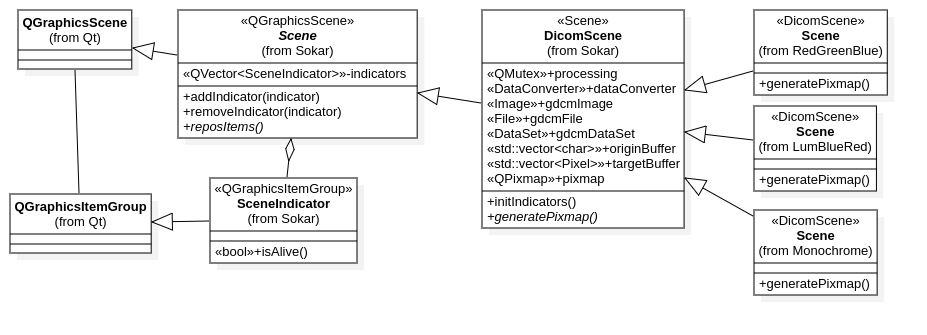
\includegraphics[width=\textwidth]{img/uml/dicom-scene.png}
    \caption{Diagram klas UML dziedziczenia klasy \sokarclass{DicomScene}.}
    \label{uml:sokar-dicomscene}
\end{figure}

\subsubsection{Wyświetlanie sceny}
\par
Qt zapewnia własny silnik graficzny, który pozwala na łatwą wizualizację przedmiotów, z obsługą obrotu i powiększania.
Silnik ten jest implementowany w postaci scen za pomocą \qtclass{QGraphicsScene}.
Natomiast klasa \qtclass{QGraphicsView} dostarcza element interfejsu graficznego, który jest miejscem do wyświetlania scen.
\par
Na scenie mogą być wyświetlane obiekty dziedziczące po \qtclass{QGraphicsItem}.
Obiekty te mogą być dodawane, usuwane i przesuwane ze sceny w czasie rzeczywistym.
Dodatkowo można na tych obiektach używać przekształceń macierzowych we współrzędnych jednorodnych, szerzej opisanych w sekcji \ref{sec:algorithm-pixmap-transformat}.
Przykłady obiektów używanych w scenie \sokarclass{DicomScene}:
\begin{itemize}
    \item \qtclass{QGraphicsTextItem} --- element wyświetlający tekst.
          Obsługuje on możliwość wyświetlania podstawowych znaczników HTML.
    \item \qtclass{QGraphicsLineItem} --- element wyświetlający prostą linię z punktu $A$ do $B$
    \item \qtclass{QGraphicsPixmapItem} --- element wyświetlający obrazy graficzne, obiekty klasy \qtclass{QPixmap}
    \item \qtclass{QGraphicsItemGroup} --- element grupujący wiele elementów.
          Pozwala na łatwą implementację bardziej złożonych struktur
\end{itemize}
\par
Silnik graficzny Qt został rozszerzony o dodatkowe możliwości ułożone w warstwy.
Pierwszą warstwą jest biblioteka Qt (\qtclass{QGraphicsScene}).
Drugą jest scena z elementami, które same są w stanie się przemieszczać po scenie (\sokarclass{Scene}).
Trzecia warstwa to scena z obrazem \DICOM (\sokarclass{DicomScene}).
\par
W pierwszej warstwie elementy graficzne zostały zaimplementowane za pomocą klasy \sokarclass{SceneIndicator}, dziedziczącej po \qtclass{QGraphicsItemGroup}.
Sceny zostały zaimplementowane za pomocą klasy \sokarclass{Scene}, dziedziczącej po \qtclass{QGraphicsScene}.
Kontrolka graficzna została zaimplementowana za pomocą klasy \sokarclass{DicomGraphics}, dziedziczącej po \qtclass{QGraphicsView}.
\par
W Qt sceny wyświetlające elementy nie rozróżniają wielkości kontrolki graficznej, która je wyświetla, dodatkowo nie wiedzą czy są wyświetlane czy nie.
Obiekty klasy \sokarclass{DicomGraphics}, informują sceny, o wielkości kontrolki i o zmianach tej wielkości.
Dodatkowo obiekty \sokarclass{SceneIndicator} otrzymują informacje o zmianach wielkości scen i są wstanie same zmieniać swoją pozycję na scenie poprzez wirtualną funkcję \sokarfunction{SceneIndicator}{reposition}.
\par
W trzeciej warstwie została dodana klasa \sokarclass{DicomScene} dziedzicząca po \sokarclass{Scene}.
\par
Diagram klas UML znajduje się na rysunku \ref{uml:sokar-scene-layers}.

\begin{figure}[!htbp]
    \centering
    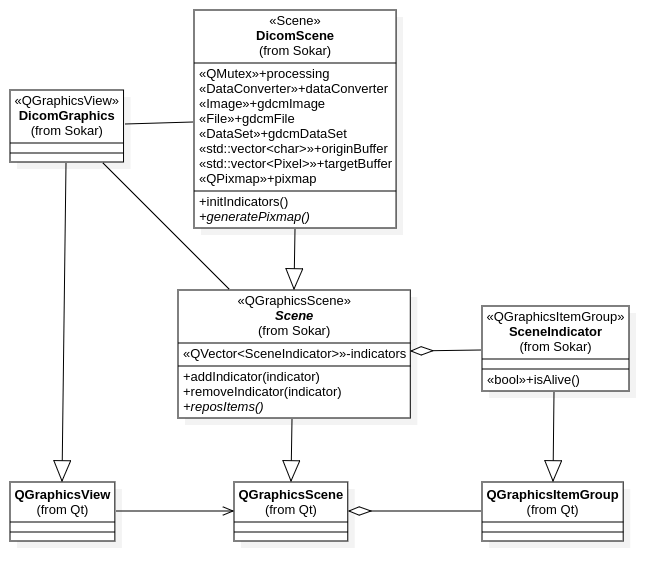
\includegraphics[width=\textwidth]{img/uml/dicom-scene-layers.png}
    \caption{Diagram klas UML dziedziczenia klasy \sokarclass{DicomScene}.}
    \label{uml:sokar-scene-layers}
\end{figure}


\subsubsection{Informacje wyświetlane na scenie}

\par
Wszystkie elementy wyświetlające dane z pliku \DICOM dziedziczą po klasie \sokarclass{SceneIndicator}.
Diagram klas UML znajduje się na rysunku \ref{uml:sokar-scene-indicators}.

\begin{figure}[!htbp]
    \centering
    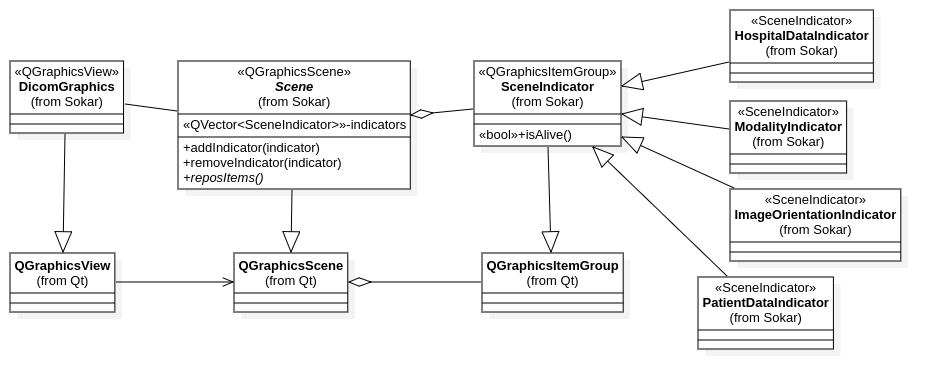
\includegraphics[width=\textwidth]{img/uml/dicom-scene-indicators.png}
    \caption{Diagram klas UML dziedziczenia klasy \sokarclass{SceneIndicator}.}
    \label{uml:sokar-scene-indicators}
\end{figure}

\par
Domyślnie obiekty wyświetlające informacje (tytuły punktów to nazwy klas):

\paragraph{Dane pacjenta}

Dane pacjenta są implementowane przez \sokarclass{PatientDataIndicator} i pojawiają się zawsze na scenie w lewym górnym rogu.
Zawierają następujące linie:
\begin{itemize}
    \item Nazwa pacjenta oraz płeć

          Nazwa pacjenta znajduje się w \dicomtag{Patient Name}{0010}{0010} o \dicomvr{PN}.

          Płeć, zapisana jest w \dicomtag{Patient Sex}{0010}{0040} i może mieć następujące wartości:
          \begin{itemize}
              \item \dataword{M } --- oznacza mężczyznę, wyświetlana jako znak \utfMaleSign,
              \item \dataword{F } --- oznacza kobietę, wyświetlana jako znak \utfFemaleSign,
              \item \dataword{O } --- oznacza inną płeć i nie jest wyświetlana.
          \end{itemize}

          Przykład: \enquote{Jan Nowak \utfMaleSign}.

    \item Identyfikator pacjenta

          Unikalny identyfikator pacjenta ze znacznika \dicomtag{Patient ID}{0010}{0020} wyświetlany jest w takiej formie, w jakiej jest zapisany.
          W praktyce najczęściej jest to numer z systemu używanego w danym szpitalu, rzadziej numer PESEL.

          Przykład: \enquote{HIS/000000}.

    \item Data urodzenia oraz wiek pacjenta w trakcie badania

          Data urodzenia znajdująca się w \dicomtag{Patient Birth Date}{0010}{0030} i jest zamieniana na format \dataword{YYYY-MM-DD}.
          Dodatkowo, jeżeli tag \dicomtag{PatientAge}{0010}{1010} jest obecny, wyświetlany jest także wiek pacjenta w czasie badania.

          Przykład: \enquote{born 1982-08-09, 28 years}.

    \item Opis lub klasyfikacja badania dokonana przez instytucję

          Tekst brany z \dicomtag{Study Description}{0008}{1030} i wyświetlany bez ingerencji.

          UWAGA: Ta wartość jest wpisywana przez technika, operatora lub lekarza wykonującego badanie, więc wartość ta może być nieprzewidywalna.

    \item Opis serii

          Tekst brany z \dicomtag{Series Description}{0008}{103E} i wyświetlany bez ingerencji.

          UWAGA: Ta wartość jest wpisywana przez technika, operatora lub lekarza wykonującego badanie, więc wartość ta może być nieprzewidywalna.
\end{itemize}

Przykład pełnego teksu:

\begin{center}
    \begin{tabular}{l}
        \textbf{Jan Nowak} \utfMaleSign \\
        HIS/123456                              \\
        born 1996-01-01, 19 years               \\
        Kregoslup ledzwiowy a-p + boczne        \\
        AP
    \end{tabular}
\end{center}

\paragraph{Dane jednostki organizacyjnej}

Dane jednostki organizacyjnej są implementowane przez \sokarclass{HospitalDataIndicator}.
Pojawiają się zawsze na scenie w prawym górnym rogu i zawierają następujące linie:
\begin{itemize}
    \item Nazwa instytucji

          Tekst jest obierany z \dicomtag{Institutional Department Name}{0008}{1040} i wyświetlany bez ingerencji.

    \item Producent wyposażenia wraz z modelem urządzenia

          Tekst jest obierany z \dicomtag{Manufacturer}{0008}{0070} i \dicomtag{Manufacturer Model Name}{0008}{1070}, oddzielony spacją i wyświetlany bez ingerencji.

    \item Nazwisko lekarza wykonującego badanie

          Tekst jest obierany z \dicomtag{Referring Physician Name}{0008}{0090} i wyświetlany bez ingerencji.

    \item Nazwisko operatora wspierającego badanie

          Tekst jest obierany z \dicomtag{Operators Name}{0008}{1070} i wyświetlany bez ingerencji.
\end{itemize}

\paragraph{Orientacja obrazu}

\par
Orientacja obrazu jest implementowana przez \sokarclass{ImageOrientationIndicator}.
Obiekt wyświetla cztery litery oznaczające orientację obrazu w stosunku do pacjenta.
Obiekt posiada cztery pola: lewe, górne, prawe i dolne.

\par
Każda z sześciu możliwych liter oznacza kierunek oraz zwrot w jakim jest ułożony pacjent:
\begin{itemize}
    \item \enquote{R} --- right --- część prawa pacjenta,
    \item \enquote{L} --- left --- część lewa pacjenta,
    \item \enquote{A} --- anterior --- przód pacjenta,
    \item \enquote{P} --- posterior --- tył pacjenta,
    \item \enquote{F} --- feet --- część dolna pacjenta,
    \item \enquote{H} --- head --- część górna pacjenta.
\end{itemize}

\par
Pełny opis implementacji algorytmu wyznaczania stron znajduje się w sekcji \ref{sec:algorithm-imageorientationindicator}.

\paragraph{Podziałka}

Podziałka Jest implementowana przez \sokarclass{PixelSpacingIndicator}.
Obiekt wyświetla podziałkę informującą o rzeczywistych rozmiarach obiektu na obrazie.
Pojawiają się na dole i po prawej stronie sceny, gdy znacznik \dicomtag{PixelSpacing}{0028}{0030} jest obecny.
Wygląd podziałki można zaobserwować na rysunku \ref{fig:imageorientationindicator1}.

Podziałka dostosowuje swoją wielkość do obecnej sceny, jak i do innych elementów na scenie.
Wartości wyświetlane biorą pod uwagę transformatę skali i rotacji obrazu.

\paragraph{Dodatkowe informacje o modalności}

Te informacje są implementowane przez \sokarclass{ModalityIndicator}.
Obiekt wyświetla informacje o akwizycji obrazu.
Dane różnią się w zależności od modalności obrazu.
Domyślnie zawierają następujące linie:
\begin{itemize}
    \item \enquote{Modality} --- modalność --- pobierana ze znacznika \dicomtag{Modality}{0008}{0060},
    \item \enquote{Series} --- numer serii --- pobierany ze znacznika \dicomtag{Series Number}{0020}{0011},
    \item \enquote{Instance number} --- numer instancji w serii --- pobierany ze znacznika \dicomtag{Instance Number}{0020}{0013},
    \item Wartości odnoszące się do właściwości plastra obrazu:
          \enquote{Slice thickness} --- grubość plastra --- pobierana ze znacznika \dicomtag{Slice Thickness}{0018}{0050},
          \enquote{Slice location} --- pozycja plastra --- pobierana ze znacznika \dicomtag{Slice Location}{0020}{1041}.
\end{itemize}

W przypadku następujących modalności zawierają również następujące informacje:
\begin{itemize}
    \item CT --- tomografia komputerowa:
          \begin{itemize}
              \item \enquote{KVP} --- szczytowe napięcie wyjściowe generatora promieniowania rentgenowskiego --- wyrażone w kilovoltach, pobierane z \dicomtag{KVP}{0018}{0060}
              \item \enquote{Exposure time} --- czas ekspozycji --- pobierany ze znacznika \dicomtag{Exposure Time}{0018}{1150}.
              \item \enquote{Exposure} --- ekspozycja --- wyrażona w $mAs$, pobierana ze znacznika \dicomtag{Exposure}{0018}{1152}.
          \end{itemize}

    \item RT/CR --- radiologia analogowa i cyfrowa:
          \begin{itemize}
              \item \enquote{Exposure time} --- czas ekspozycji --- pobierany ze znacznika \dicomtag{Exposure Time}{0018}{1150}.
              \item \enquote{KVP} --- szczytowe napięcie wyjściowe generatora promieniowania rentgenowskiego wyrażone w kilovoltach, pobierane z \dicomtag{KVP}{0018}{0060}
          \end{itemize}

    \item MR --- rezonans magnetyczny:
          \begin{itemize}
              \item \enquote{Repetition time} --- czas repetycji --- pobierany ze znacznika \dicomtag{Repetition Time}{0018}{0080}.
              \item \enquote{Echo time} --- czas echa --- pobierany ze znacznika \dicomtag{Echo Time}{0018}{0081}.
              \item \enquote{Magnetic field} --- pole magnetyczne --- nominalna wartość pola magnetycznego wyrażona w teslach pobierana ze znacznika \dicomtag{Magnetic Field Strength}{0018}{0087}.
              \item \enquote{SAR} --- swoiste tempo pochłaniania energii --- pobierane ze znacznika \dicomtag{SAR}{0018}{1316}.
          \end{itemize}
\end{itemize}

\subsubsection{Generowanie obrazów z danych}

Klasa \sokarclass{DicomScene} jest klasą abstrakcyjną i nie generuje obrazu.
Pozostawia to klasom dziedziczącym po niej.
Dokładna analiza cyklu generowania obrazów jest opisana w sekcji \ref{sec:algorithm-pixmap-generate}.

\subsubsection{Przekształcenia macierzowe obrazu}

\par
Wyświetlanie obrazu na scenie odbywa sie za pomocą obiektu klasy \qtclass{QGraphicsPixmapItem}, który dziedziczy po \qtclass{QGraphicsItem}.
Ta ostatnia klasa ma w sobie zaimplementowaną funkcję pozwalającą na nałożenie przekształcenia macierzowego na obraz.
W Qt przekształcenia macierzowe są implementowane za pomocą klasy \qtclass{QTransform}, która jest macierzą 3 na 3.

Zostały zdefiniowane 4 macierze, które działają na obiekt obrazu wyświetlanego na scenie:
\begin{itemize}
    \item \cppcode{centerTransform} --- macierz wyśrodkowująca (zadaniem tego przekształcenia jest przeniesienie obrazu na środek sceny)
    \item \cppcode{panTransform} --- macierz przesunięcia
    \item \cppcode{scaleTransform} --- macierz skali
    \item \cppcode{rotateTransform} --- macierz rotacji
\end{itemize}

\par
Podczas interakcji z użytkownikiem macierze mogą ulegać zmianom na dwa sposoby.
Pierwszym sposobem jest odebranie sygnału od przycisków z paska zadań, szerzej opisanego w sekcji \ref{sec:sokar-dicomtoolbar}, znajdującego się nad sceną.
Drugi sposób to przechwycenie ruchów myszki, gdy wciśnięty jest lewy przycisk myszy.
\par
Pełny algorytm tworzenia macierzy i ich zmian poprzez interakcje z użytkownikiem, znajduje się w sekcji \ref{sec:algorithm-pixmap-transformat}.

\subsection{Kolekcje scen}
\label{sec:sokar-scenesets}

Abstrakcyjna klasa \sokarclass{DicomSceneSet} implementuje wektor scen za pomocą klasy \qtclass{QVector}.
Jest to obiekt, który przechowuje sceny i tworzy sekwencje scen, która jest rzeczywistym ułożeniem ramek obrazów.
Są dwie implementacje kolekcji scen: kolekcja plików i kolekcja ramek z jednego pliku.
Diagram klas UML znajduje się na rysunku \ref{uml:sokar-scene-sets}.

\begin{figure}[!htbp]
    \centering
    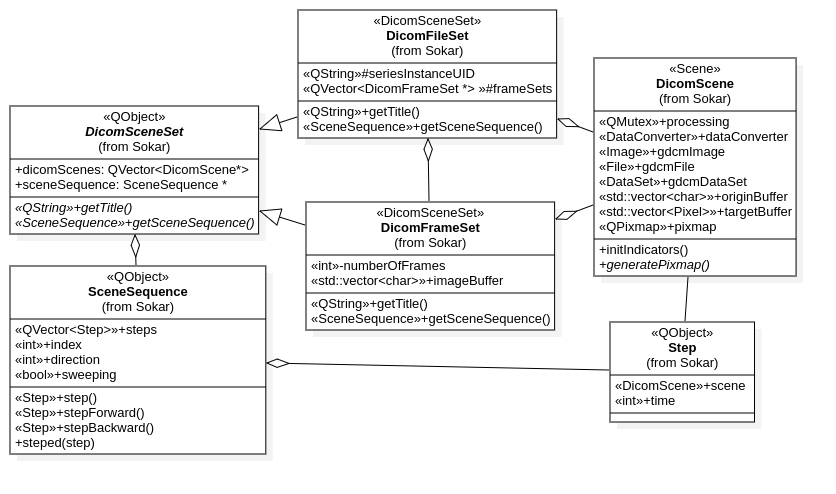
\includegraphics[width=\textwidth]{img/uml/sokar-scene-sets.png}
    \caption{Diagram klas UML dziedziczenia klasy \sokarclass{DicomScene}.}
    \label{uml:sokar-scene-sets}
\end{figure}

\subsubsection{Sekwencja scen}
\label{sec:sokar-scenesequence}

\par
Sekwencja scen implementuje strukturę danych informującą o przejściach pomiędzy scenami poprzez klasę \sokarclass{SceneSequence}.
Sekwencja to wektor zawierający kroki z dodatkowymi informacjami o stanie sekwencji:
\begin{itemize}
    \item indeks, w którym obecnie znajduje się sekwencja
    \item kierunek sekwencji --- sekwencja może iść w stronę początku lub końca
    \item rodzaj przemiatania --- wartość logiczna informująca w jaki sposób ma zachować się, gdy sekwencja dojdzie do końca, lub początku
\end{itemize}
Po dojściu do końca sekwencja skoczy do pierwszego elementu lub może zmienić kierunek i zacząć iść do tyłu.

\par
Kroki implementowane przez klasę \sokarclass{Step} zawierają następujące informacje: wskaźnik do sceny oraz czas trwania sceny.

\par
Sekwencja ma wbudowane funkcje zapewniające przesuwanie się po indeksie na wektorze:
\begin{itemize}
    \item \sokarfunction{SceneSequence}{stepForward} --- krok do przodu, zwiększa indeks tym samym wykonując krok w stronę końca sekwencji
    \item \sokarfunction{SceneSequence}{stepBackward} --- krok do tyłu, zmniejsza indeks tym samym wykonując krok w stronę początku sekwencji
    \item \sokarfunction{SceneSequence}{step} --- wykonuje krok w tył lub przód w zależności od kierunku sekwencji
\end{itemize}
Wszystkie powyższe funkcje są zarazem slotami dla sygnałów oraz emitują sygnał \sokarfunction{SceneSequence}{steped}.

\subsubsection{Kolekcja ramek DICOM}
\label{sec:sokar-dicomframeset}

\par
Zbiory ramek są implementowane przez \sokarclass{DicomFrameSet} i są tworzone z jednego wczytanego pliku DICOM.
Klasa tworzy obiekt konwertera i pobiera liczbę ramek w obrazie.
Tworzy jeden buffor na wszystkie ramki obrazów, a następnie dzieli go na ilość ramek.
Biblioteka GDCM nie daje dostępu do oryginalnego bufora, dlatego wymagany jest bufor pośredni.
Następnie jest tworzonych tyle obiektów scen ile jest ramek.
\par
Kolejność sekwencji scen jest taka sama jak kolejność ramek.
Natomiast czas wyświetlania ramki może być zapisany w różnych znacznikach.
To, w którym znaczniku został zapisany, informuje element o znaczniku \dicomtag{Frame Increment Pointer}{0028}{0009}.
Zawiera on wskaźnik do elementu o zadanym znaczniku.
\par
Została zaimplementowana obsługa poniższych znaczników:
\begin{itemize}
    \item \dicomtag{Frame Time}{0018}{1063} --- element z tym znacznikiem zawiera czas trwania jednej ramki w milisekundach, każdemu krokowi jest przypisywana ta wartość trwania

    \item \dicomtag{Frame Time Vector}{0018}{1065} --- zawiera tablice z przyrostami czasu w milisekundach między n-tą ramką a poprzednią klatką. Pierwsza ramka ma zawsze przyrost czasu równy 0.
    
    \item \dicomtag{Cine Rate}{0018}{0040} --- zawiera ilość klatek wyświetlanych na sekundę, każdemu krokowi jest przypisywana wartość do niej odwrotna.
\end{itemize}
W przypadku braku znacznika lub gdy zostaje wskazany znacznik nieznany, czas trwania ramki wynosi $83.3$ milisekundy, co odpowiada 12 klatkom na sekundę.


\subsubsection{Kolekcja plików DICOM}
\label{sec:sokar-dicomfileset}
\par
Zbiory plików są implementowane przez \sokarclass{DicomFileSet} i służą do przechowywania wielu wczytanych plików DICOM.
Na początku pliki są sortowane na podstawie liczby zawartej w elemencie o znaczniku \dicomtag{Instance Number}{0020}{0x0013}.
Dla każdego pliku jest tworzony obiekt \sokarclass{DicomFrameSet}.
\par
Sekwencja jest tworzona poprzez połączenie sekwencji poszczególnych obrazów.

\subsubsection{Segregowanie obrazów}
\label{sec:sokar-dicomfileset-create}
\par
W przypadku kiedy mamy do czynienia z wieloma plikami, należy jest rozdzielić na serie i uporządkować w odpowiedniej kolejności.
Unikalny identyfikator serii jest zawarty w elemencie danych znaczniku \dicomtag{Series Instance UID}{0020}{000E}.
Kolejności obrazów w serii to liczba zawarta w elemencie danych o znaczniku \dicomtag{Instance Number}{0020}{0x0013}.
\par
Segregacja odbywa się za pomocą funkcji \sokarfunction{DicomFileSet}{create}.
Do funkcji jest przesyłany wektor z wczytanymi plikami DICOM, następnie dzieli ona pliki na zbiory zawierające zdjęcia tej samej serii, tworzy obiekty zbiorów plików DICOM, ostatecznie zwraca ona wektor z gotowymi obiektami zbiorów plików DICOM.
Sortowanie plików DICOM według ich kolejności odbywa się za pomocą funkcji \stdclass{sort}{algorithm/sort} wewnątrz konstruktora klasy \sokarclass{DicomFileSet}, który nie jest publiczny.

\subsection{Zakładka}
\label{sec:sokar-dicomview}
\par
Każda zakładka z obrazem lub obrazami jest implementowana przez klasę \sokarclass{DicomView}.

\par
Interfejs graficzny \sokarclass{DicomView} wyświetla następujące elementy:
\begin{itemize}
    \item pasek narzędzi znajdujący się na górze - implementowany za pomocą klasy \sokarclass{DicomToolBar}, opisany w sekcji \ref{sec:sokar-dicomtoolbar}
    \item miejsce na scene z obrazem DICOM na środku - implementowany za pomocą klasy \sokarclass{DicomGraphics}, opisany w sekcji \ref{sec:sokar-dicomgraphics}
    \item suwak filmu w dolnej części - implementowany za pomocą klasy \sokarclass{MovieBar}, opisany w sekcji \ref{sec:sokar-moviebar}
    \item podgląd miniaturek obrazów w prawej części - implementowany za pomocą klasy \sokarclass{FrameChooser}, opisany w sekcji \ref{sec:sokar-framechooser}
\end{itemize}

\par
Dodatkowo posiada obiekt \sokarclass{DicomSceneSet}, który jest zbiorem obrazów opisany w sekcji \ref{sec:sokar-scenesets}.
\sokarclass{DicomView} łączy zdarzenia wysyłane przez wszystkie obiekty.

\par
Poniżej jest opisane zachowanie tych elementów:

\subsubsection{Elementy interfejsu graficznego}

\begin{figure}[!htbp]
    \centering
    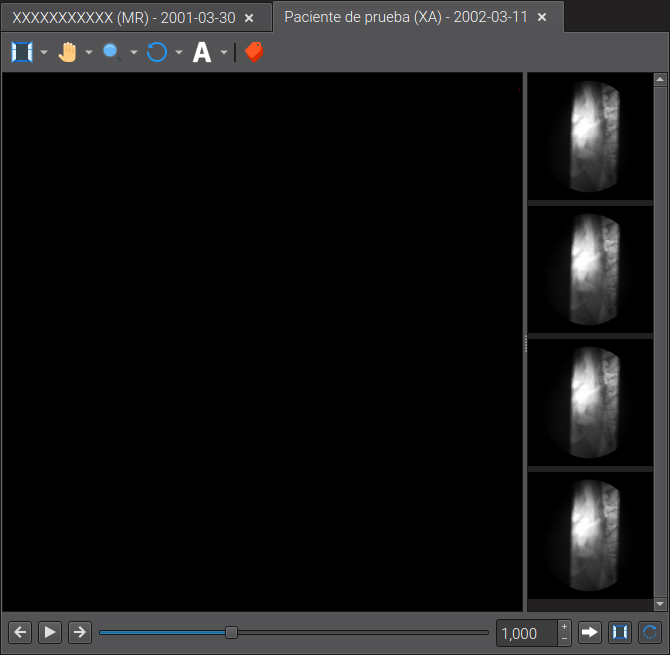
\includegraphics[width=\textwidth]{img/sokar-dicomview-001.png}
    \caption{Wygląd DicomView wraz z numeracją elementów interfejsu. Zdjęcie własne.}
    \label{fig:sokar-dicomview001}
\end{figure}

\paragraph{\sokarclass{DicomToolBar}}
\label{sec:sokar-dicomtoolbar}
\label{sec:sokar-dicomtoolbar}
\par
Pasek narzędzi znajdujący się na górze, implementowany przez klasę \sokarclass{DicomToolBar}, dziedziczącą po klasy \qtclass{QToolBar}.
Posiada on zespół ikonek z rozwijalnymi menu kontekstowymi.

\par
Kliknięcie odpowiedniej ikony spowoduje wysłanie sygnału do obecnie wyświetlanej sceny.
Są dwa sygnały możliwe do wysłania \sokarfunction{DicomToolBar}{stateToggleSignal} lub \sokarfunction{DicomToolBar}{actionTriggerSignal}.
Pierwszy sygnał oznacza zmianę stanu paska, czyli sposób obsługi myszki, zawierał jeden argument: stan (typu \cppcode{enum}).
Sygnał ten okazał się bez użyteczny i nie jest wykorzystywany przez scene.
Drugi oznacza akcje, sygnał akcji, która powinna być wykonana na przez scenę, zawiera dwa argumenty: typ akcji (typu \cppcode{enum}) i stan akcji (typu \cppcode{bool} z domyślną wartością \cppcode{false}).

Ikony na pasku:
\begin{itemize}
    \item Okienkowanie (1)

          Stan: \cppcode{Windowing}.
          Oznacza, że horyzontalny ruch myszki powinien zmieniać szerokość okna, a wertykalny środek okna.
          Przycisk jest aktywny tylko wtedy gdy na obecna scena posiada obraz monochromatyczny.

    \item Przesuwanie (2)

          Stan: \cppcode{Pan}.
          Oznacza, że ruch myszki powinien przesuwać obraz na scenie w prawo, lewo, góra, dół, kiedy jest wciśnięty klawisz myszy.

          Rozwijalne menu zawiera tylko jedne element \enquote{Move To Center} wysyłający sygnał akcji z argumentem \cppcode{ClearPan}.

    \item Skalowanie (3)

          Stan: \cppcode{Zoom}.
          Oznacza, że ruch myszki powinien skalować obraz kiedy jest wciśnięty klawisz myszy.

          Menu rozwijalne:
          \begin{itemize}
              \item Fit To Screen --- Dopasuj do ekranu

                    Akcja: \cppcode{Fit2Screen}.

                    Po otrzymaniu sygnału obraz na scenie powinien dopasować swoją wielkość do wielkości sceny

              \item Original Resolution --- Skala jeden do jednego

                    Akcja: \cppcode{OriginalResolution}.

                    Po otrzymaniu sygnału obraz na scenie powinien dopasować swoją wielkość jeden do jedne w stosunku do piksela na ekranie.

          \end{itemize}

    \item Rotacja (4)

          Stan: \cppcode{Rotate}.
          Oznacza, że ruch myszki powinien obracać obrazem znajdującym się na scenie.

          Menu rozwijalne:
          \begin{itemize}
              \item Rotate Right --- Obróć w prawo

                    Akcja: \cppcode{RotateRight90}.

                    Po otrzymaniu sygnału obraz na scenie powinien obróć się o 90 stopni w prawo.

              \item Rotate Left --- Obróć w lewo

                    Akcja: \cppcode{RotateLeft90}.

                    Po otrzymaniu sygnału obraz na scenie powinien obróć się o 90 stopni w lewo.

              \item Flip Horizontal --- Odbij lustrzanie poziomo

                    Akcja: \cppcode{FlipHorizontal}.

                    Po otrzymaniu sygnału obraz na scenie powinien odbić się lustrzanie poziomo.

              \item Flip Vertical --- Odbij lustrzanie pionowo

                    Akcja: \cppcode{FlipVertical}.

                    Po otrzymaniu sygnału obraz na scenie powinien odbić się lustrzanie pionowo.

              \item Clear Transformation --- Wyczyść przekształcenia obrotu

                    Akcja: \cppcode{ClearRotate}.

                    Po otrzymaniu sygnału obraz na scenie powinien wyczyścić transformatę obrotu.

          \end{itemize}
    \item Informacje na obrazie (5)

          Ten element potrafi wyłączyć wyświetlanie niektórych elementów na scenie.
          Kliknięcie go odznacza lub zaznacza wszystkie pozycje w menu kontekstowym.
          Wszystkie pozycje są pozycjami odznaczanymi.

          Menu rozwijalne:
          \begin{itemize}
              \item Patient Data --- Dane pacjenta

                    Akcja: \cppcode{PatientData}.

                    Po otrzymaniu sygnału obiekt klasy \sokarclass{PatientDataIndicator} znajdujący się na scenie powinien pokazać lub ukryć się w zależności od stanu pozycji.

              \item Hospital Data --- Dane szpitala

                    Akcja: \cppcode{HospitalData}.

                    Po otrzymaniu sygnału obiekt klasy \sokarclass{HospitalDataIndicator} znajdujący się na scenie powinien pokazać lub ukryć się w zależności od stanu pozycji.
              \item Image Acquisition --- Dane akwizycji

                    Akcja: \cppcode{ModalityData}.

                    Po otrzymaniu sygnału obiekt klasy \sokarclass{ModalityIndicator} znajdujący się na scenie powinien pokazać lub ukryć się w zależności od stanu pozycji.

          \end{itemize}

    \item Tagi (5)

          Akcja: \cppcode{OpenDataSet}.

          Kliknięcie tego przycisku wyśle prośbę o otworzenie okna ze zbiorem elementów danych pliku obrazu, który jest obecnie wyświetlany na scenie.

\end{itemize}

\paragraph{\sokarclass{DicomGraphics}}
\label{sec:sokar-dicomgraphics}

\paragraph{\sokarclass{MovieBar}}
\label{sec:sokar-moviebar}

\par
Jest paskiem filmu w dolnej części \sokarclass{DicomView}.
Element graficzny ma dostęp do sekwencji scen i ukrywa swoją obecność przed użytkownikiem, kiedy w sekwencji jest tylko jedna scena.

\par
Pasek jest podzielony na trzy części: trzy przyciski znajdujące się po lewej, pasek pokazujący postępu sekwencji na środku i prządka z trzema przyciskami po prawej.

\par
Trzy lewe przyciski odpowiadają za poruszanie się po sekwencji.
Wciśniecie pierwszego przycisku (z indeksem 8 na rysunku \ref{fig:sokar-dicomview001}) powoduje zatrzymanie upływu sekwencji i wysłanie sygnału \sokarfunction{SceneSequence}{stepBackward} do sekwencji.
Wciśniecie drugiego przycisku (9) powoduje włączenie lub wyłączenie upływu sekwencji.
Wciśniecie trzeciego przycisku (10) powoduje zatrzymanie upływu sekwencji i wysłanie sygnału \sokarfunction{SceneSequence}{stepForward} do sekwencji.
\par
Pasek (11) pokazujący postępu sekwencji jest obiektem klasy \qtclass{QSlider}.
Odświeżanie paska jest wrażliwe na sygnał \sokarfunction{SceneSequence}{steped} of sekwencji.
\par
Elementy po prawej stronie definiuje parametry trybu filmowego.
Prządka (12), element do wprowadzania liczby zmiennoprzecinkowej klasy \qtclass{QDoubleSpinBox}.
Im większa wartość liczby tym klatki filmu są dłużej wyświetlane.
Drugi (13) przycisk pozwala zmienić sposób przemiatania.
Trzeci (14) przycisk wymusza tryb jednego okna dla wszystkich klatek filmu.
Jeżeli mamy załadowanych wile obrazów tego samego badania, to nie koniecznie muszą mieć to samo okno.
Dodatkowo ten tryb pozwala wprowadzić jednolite okienko dla wszystkich klatek po zmianie parametrów tego okienka na jednej klatce.
Czwarty (15) i ostatni przycisk służy do użycia jednej macierzy transformaty na wszystkich klatkach.

\subparagraph*{Tryb filmowy}

\par
Tryb filmowy można aktywować jedynie wtedy gdy w sekwencji scen jest więcej niż jedna scena.
Włączenie trybu filmowego polega na stworzeniu obiektu klasy \sokarclass{MovieMode}.
Obiekt ten zapisuje wskaźnik go obecnie wyświetlanej sceny, to czy powinno być użyte to samo okno, oraz to czy powinna być używana ta sama transformata.
Następnie obiekt ten jest wysyłany do wszystkich scen w sekwencji.
Uruchamiany jest timer, obiekt klasy \qtclass{QTimer}, na czas równy czasu trwania sceny zapisanego w kroku przemnożonego przez liczbę z prządki.
Po upływie timera, wstawiana jest nowa scena za pomocą sygnały \sokarfunction{MovieBar}{setStep}, a timer jest ustawiany nan nowo.

\paragraph{\sokarclass{FrameChooser}}
\label{sec:sokar-framechooser}

Ten element to wybór scen za pomocą ikon, implementowany przez klasę \sokarclass{DicomView}.
Element, podobnie jak pasek filmu ma dostęp do sekwencji scen i ukrywa swoją obecność przed użytkownikiem, kiedy w sekwencji jest tylko jedna scena.
Po wciśnięciu ikony jest zmieniana scena.

\subsection{Obiekt zakładek}
\label{sec:sokar-dicomtabs}

\par
Obiekt zakładek, implementowany za pomocą klasy \sokarclass{DicomTabs}, odpowiada za wyświetlanie wielu obiektów zakładek w jednym obiekcie interfejsu.
Obsługuje również wczytanie nowych plików.

\subsubsection{Sposoby uzyskania nowych plików}

\par
Otworzenie nowego pliku może odbyć się z następujących źródeł: obiektu drzewa ze strukturą plików w systemie (opisanego w \ref{sec:sokar-framechooser}), menu programu (opisanego w \ref{sec:sokar-window-menu}), lub poprzez przeciągnięcie i upuszczenie pliku.
Z dwóch pierwszych można wczytać tylko po jednym pliku, natomiast trzecim sposobem można wczytać zarówno jeden jak i wiele plików.
Wysyłanie prośby odbywa się za pomocą dwóch funkcji: \sokarfunction{DicomTabs}{addDicomFile} i \sokarfunction{DicomTabs}{addDicomFiles}.
Każda z tych funkcji ma dwa przeciążenia, jedno z parametrem ścieżki a drugie z wczytanym plikiem.

\subsubsection{Wczytywanie plików}

\par
Po dostarczeniu ścieżek do obiektu, pliki zostają wczytane za pomocą funkcji \gdcmclass{ImageReader}.
W przypadku błędu proces wczytywania się kończy.
Po wczytaniu wszystkich plików zostaje utworzony obiekt kolekcji ramek obrazu lub kolekcji plików \DICOM za pomocą funkcji \sokarfunction{DicomFileSet}{create}, opisanej w sekcji \ref{sec:sokar-dicomfileset-create}.


\subsection{Okno główne programu}
\label{sec:sokar-window}

\par
Główne okno programu jest implementowane przez \sokarclass{MainWindow}.
Jest wywoływane od razu po uruchomieniu programu.
\par
Zawiera w sobie 4 elementy: menu, drzewo ze strukturą plików, obiekt z zakładkami i sugestie, aby nie używać programu w celach medycznych w dolnej części okna.

\subsubsection{Drzewo katalogów i zakładki}

\par
W lewej części okna znajduje się element listy, implementowany przez \sokarclass{FileTree}, zawiera on w sobie model drzewa plików systemu, który z kolei jest implementowany przez klasę \qtclass{QFileSystemModel}.
Po wybraniu pliku, ścieżka jest przesyłana do obiektu z zakładkami.
\par
W środkowej części programu znajduje się obiekt z zakładkami, szczegółowo opisany w sekcji \ref{sec:sokar-dicomtabs}.

\subsubsection{Menu programu}
\label{sec:sokar-window-menu}

\par
W górnej części okna programu znajduje się menu, obiekt klasy \sokarclass{QMenuBar}.
Struktura Menu programu:
\begin{itemize}
    \item File
          \begin{itemize}
              \item Open --- otwiera okienko wyboru plików, implementowane przez \qtfunction{QFileDialog}{getOpenFileName}, następnie wczytuje plik
              \item Open Recent --- program zapisuje ostatnio wczytane pliki i pozwala ja ich ponowne wczytanie z tego menu
              \item Export as --- zapisanie obrazu w formacie JPEG, BMP, GIF lub PNG.
                    Zapisywanie jest zaimplementowane przez funkcje \qtfunction{QImage}{save}, która umożliwia zapisanie obrazu do pliku.
              \item Exit --- wyjście z aplikacji
          \end{itemize}
    \item Help
          \begin{itemize}
              \item About Qt --- otwiera okno informacji o bibliotece Qt.
                    Biblioteka Qt ma wbudowane takie okno w postaci \qtfunction{QMessageBox}{aboutQt}
              \item About GDCM --- otwiera okno z informacjami o bibliotece GDCM, implementowane przez funkcje \sokarfunction{About}{GDCM}
              \item About Sokar --- otwiera okno z informacjami o aplikacji, implementowane przez funkcje \sokarfunction{About}{Sokar}
          \end{itemize}
\end{itemize}


\section{Algorytmy}


\subsection{Cykl generowania obrazów}
\label{sec:algorithm-pixmap-generate}

Klasa \sokarclass{DicomScene} dostarcza następujące obiekty do generowania obrazu:
\begin{itemize}
    \item \cppcode{processing}, obiekt klasy \qtclass{QMutex}, zamek do zablokowania podczas generowania obrazu, aby parametry obrazu nie mogły być zmieniane podczas jego generowania.

    \item \cppcode{imgDimX} zmienna typu \cppcode{uint}, oznacza szerokość obrazu w pikselach.

    \item \cppcode{imgDimY} zmienna typu \cppcode{uint}, oznacza wysokość obrazu w pikselach.

    \item \cppcode{targetBuffer} wektor docelowego obrazu RGB o długości $imgDimX*imgDimY$, typu \cppcode{std::vector<Pixel>}.

          \sokarclass{Pixel} to struktura reprezentujące piksel.
          Nie jest to w żadnym wypadku obiekt, a jedynie twór ułatwiający zarządzanie kodem.

          \begin{lstlisting}
struct Pixel {
    quint8 red = 0;   
    quint8 green = 0;    
    quint8 blue = 0;   
}\end{lstlisting}

        \par
        C++ od standardu C++03 przewiduje, że elementy znajdujące się w \stdclass{vector}{container/vector} są ułożone ciągiem, jeden za drugim.
        Dlatego odwołując się do wskaźnika pierwszego elementu w ten sposób \cppcode{\&targetBuffer[0]}, mogę potraktować to jako tablicę.

    \item \cppcode{originBuffer} wektor danych wypełniona danymi z jednej ramki o długości iloczynu $imgDimX*imgDimY$ i ilości bajtów jednego piksela obrazu.

    \item \cppcode{qImage} obiekt obrazu klasy \qtclass{QImage}.

          \qtclass{QImage} można utworzyć z bufora, w tym przypadku jest to \cppcode{targetBuffer}.
          Format obrazu to \qtclass{QImage::Format\_RGB888}, czyli trzy bajty, każdy na jeden kanał.
          Proszę zwrócić uwagę, że struktura \sokarclass{Pixel} odpowiada temu formatowi.
          Według dokumentacji Qt obiekt ten po utworzeniu z istniejącego bufora powinien z niego dalej korzystać, dlatego zmiany \cppcode{targetBuffer} nie wymagają odświeżania \cppcode{qImage}.

    \item \cppcode{pixmap} obiekt obrazu do wyświetlania, klasy \qtclass{QPixmap}.

          Obiektów klasy \qtclass{QImage} nie da się wyświetlić, nie jest on przystosowany do wyświetlania.
          Natomiast klasa \qtclass{QPixmap} to reprezentacja obrazu dostosowana do wyświetlania ekranie, która może być używana jako urządzenie do malowania w bibliotece Qt.

    \item \cppcode{iconPixmap} obiekt obrazu ikonu, klasy \qtclass{QPixmap}, docelowo powinien mieć 128 pikseli na 128 pikseli.

\end{itemize}

Generowanie obrazu jest robione przez czysto wirtualną funkcje \sokarfunction{DicomScene}{generatePixmap}.
Po wywołaniu funkcji obiekt \cppcode{targetBuffer} powinien zawierać obraz wygenerowany z obecnymi parametrami.
Funkcja zwraca również wartość logiczną, który informuje nas czy \cppcode{targetBuffer} rzeczywiście został zmieniony.
Następnie obiekt \cppcode{pixmap} jest na nowo generowany na bazie \cppcode{qImage}.

Całe odświeżanie obrazu jest implementowane w funkcji \sokarfunction{DicomScene}{reloadPixmap}.
Funkcja wywołuje \sokarfunction{DicomScene}{generatePixmap} i odświeża \cppcode{pixmapItem} kiedy zajdzie taka potrzeba

Generowanie poszczególnych typów obrazów jest wyjaśnione poniżej.


\subsubsection{Obraz monochromatyczny}
\par
Obraz monochromatyczny to obraz w odcieniach szarości, od białego do czarnego lub od czarnego do białego.
Generowanie takiego obrazu odbywa się poprzez pseudokolorowanie.
Cały proces jest wyjaśniony w sekcji \ref{sec:algorithm-pixmap-monochrome}.

\subsubsection{RGB}
Obrazów zapisanych w RGB nie trzeba w żaden sposób obrabiać, dane już są prawie gotowe do wyświetlenia.
Należy je odpowiednio posortować, jeżeli zachodzi taka potrzeba.
Sposób posortowania wartości w pliku określa znacznik \dicomtag{Planar Configuration}{0x0028}{0006}.
Może on przyjąć dwie następujące wartości:

\begin{itemize}
    \item 0 --- oznacza to, że wartości pikseli są ułożone w taki sposób
        \[R_1, G_1, B_1, R_2, G_2, B_2, R_3, G_3, B_3, R_4, G_4, B_4,  ...\]
    \item 1 --- oznacza to, że wartości pikseli są ułożone w taki sposób
        \[R_1, R_2, R_3, R_4, ... , G_1, G_2, G_3, G_4, ..., B_1, B_2, B_3, B_4, ...\]
\end{itemize}
gdzie:
\begin{itemize}
    \item $R_n$ --- wartość czerwonego kanału
    \item $G_n$ --- wartość zielonego kanału
    \item $B_n$ --- wartość niebieskiego kanału
\end{itemize}

Wartości obrazu są przepisywane do \cppcode{targetBuffer} dla biblioteki QT.

\subsubsection{YBR}
\label{sec:algorithm-pixmap-ybr}

\par
YBR albo YCbCr to model przestrzeni kolorów do przechowywania obrazów i wideo.
Wykorzystuje do tego trzy typy danych: Y – składową luminancji, B lub Cb – składową różnicową chrominancji Y-B, stanowiącą różnicę między luminancją a niebieskim, oraz R lub Cr – składową chrominancji Y-R, stanowiącą różnicę między luminancją a czerwonym.
Kolor zielony jest uzyskiwany na podstawie tych trzech wartości.
YBR nie pokrywa w całości RGB, tak jak RGB nie pokrywa YBR.
Posiadają one część wspólną, co uniemożliwia wyświetlenie obrazu w stu procentach bez zniekształceń.

\par
Wartości w pliku DICOM są ułożone w taki sposób.
\[Y1, B1, R1, Y2, B2, R2, Y3, B3, R3, Y4, B4, R4,  ...\]

\par
Ponieważ wartości te reprezentują kolory, są już w pewnym sensie są obrazem, ale nie można go wyświetlić na monitorze RGB.
Dlatego należy przekonwertować kolor YBR na kolor RGB, iterując po wszystkich wartościach obrazu.

\par
Poniżej przedstawiono kod źródłowy funkcji zamiany kolory YBR na RGB.

\begin{lstlisting}
Sokar::Pixel ybr2Pixel(quint8 y, quint8 b, quint8 r) {
    qreal red, green, blue;

    red = green = blue = (255.0 / 219.0) * (y - 16.0);

    red += 255.0 / 224 * 1.402 * (r - 128);
    green -= 255.0 / 224 * 1.772 * (b - 128) * (0.114 / 0.587);
    green -= 255.0 / 224 * 1.402 * (r - 128) * (0.299 / 0.587);
    blue += 255.0 / 224 * 1.772 * (b - 128);

    /* W tym miejscu jest dokonywana utrata danych */
    red = qBound(0.0, red, 255.0);
    green = qBound(0.0, green, 255.0);
    blue = qBound(0.0, blue, 255.0);

    return Sokar::Pixel(quint8(red), quint8(green), quint8(blue));
}
\end{lstlisting}


\subsection{Generowania obrazu monochromatycznego}
\label{sec:algorithm-pixmap-monochrome}

Obraz monochromatyczny to obraz w odcieniach szarości, od białego do czarnego lub od czarnego do białego. Dane są zapisane w sposób ciągły wartość po wartości.

\subsubsection{Pseudokolorowanie obrazu}

Mamy obraz, którego piksele to n-bitowe liczby, na przykład 16 bitowa liczba całkowita.
W takiej postaci wyświetlemoe obrazu na monitorze RGB lub nawet na profesjonalnym 10-bitowym jest niemożliwe.
Należy taką liczbę przerobić na trzy liczby, reprezentujące 3 kanały RGB, czerwony, zielony i niebieski.
Dlatego do wyświetlania obrazów monochromatycznych o dużym kontraście stosuję się twór zwany okienkiem.
Jest to funkcja, która mapuje n-bitwy obraz na 8-bitowy obraz w skali szarości.
8-bitów, ponieważ monitor RGB jest wstanie wyświetlić 256 odcieni szarości.

\paragraph*{Zwiększanie kontrastu za pomocą \enquote{funkcji okna}}
Jest przyjęte, że \enquote{okno} definiuje się dwoma liczbami: środkiem, oznaczanym jako $center$ i długością, oznaczaną jako $width$.
Wyznaczamy zakres okienka $x_0$ i $x_1$ ze środka okienka $center$ i długości $width$.
\[x_0 = center - width / 2\]
\[x_1 = center + width / 2\]
Wyznaczamy parametry $a$ i $b$, prostej przechodzącej przez dwa punkty $(x_0, y_0)$ i $(x_1, y,_1)$.
Gdzie $y_0$ jest równe 0, a $y_1$ jest równe 255.
Funkcja \enquote{okna} wygląda następująco:
\[
    f(v)=
    \begin{cases}
        0     & \text{gdy $0 \le v \wedge v \le x_0$ } \\
        a*x+b & \text{gdy $x_0 < v \wedge v < x_1$}    \\
        255   & \text{gdy $x_1 \le v \wedge v \le 1$ }
    \end{cases}
\]

gdzie $v$ to wartość piksela danych obrazu.

Następnie iterujemy przez wszystkie woksele obrazu i używamy na nich funkcji \enquote{okna} i otrzymujemy obraz w skali od $0$ do $255$.
Obraz w 256 poziomach jest możliwy do wyświetlenia na obrazie RGB.
Natomiast standard \DICOM przewiduje, że obraz można jeszcze wyświetlić w wielokolorowej palecie barw.
Przykład takiej palety HotIron w porównaniu do skali szarości można zobaczyć na rysunku .
Taka paleta barw nie koniecznie musi mieć 256 odcieni, dlatego lepiej jest zrobić aby \enquote{okno}, mapowało na liczbę od 0 do 1, a później paleta mapowała na kolor RGB.



Teraz iterujemy po wszystkich możliwych wartościach wartościach obrazu i wykonujemy takie operacje.
\begin{itemize}
    \item wyznaczenie wartości okienka.
          \[y = a * x + b\]
    \item $y$ zostaje obcięte do $1.0$ lub $0.0$ jeżeli wyjdzie poza zakres od $1.0$ do $0.0$
    \item pobranie z palety pikselu odpowiadającego wartości
    \item wpisanie piksela do tablicy, tak aby najmniejsza wartości obrazu miała indeks $0$ a największy ostatni
\end{itemize}


\begin{figure}[!htbp]
    \centering
    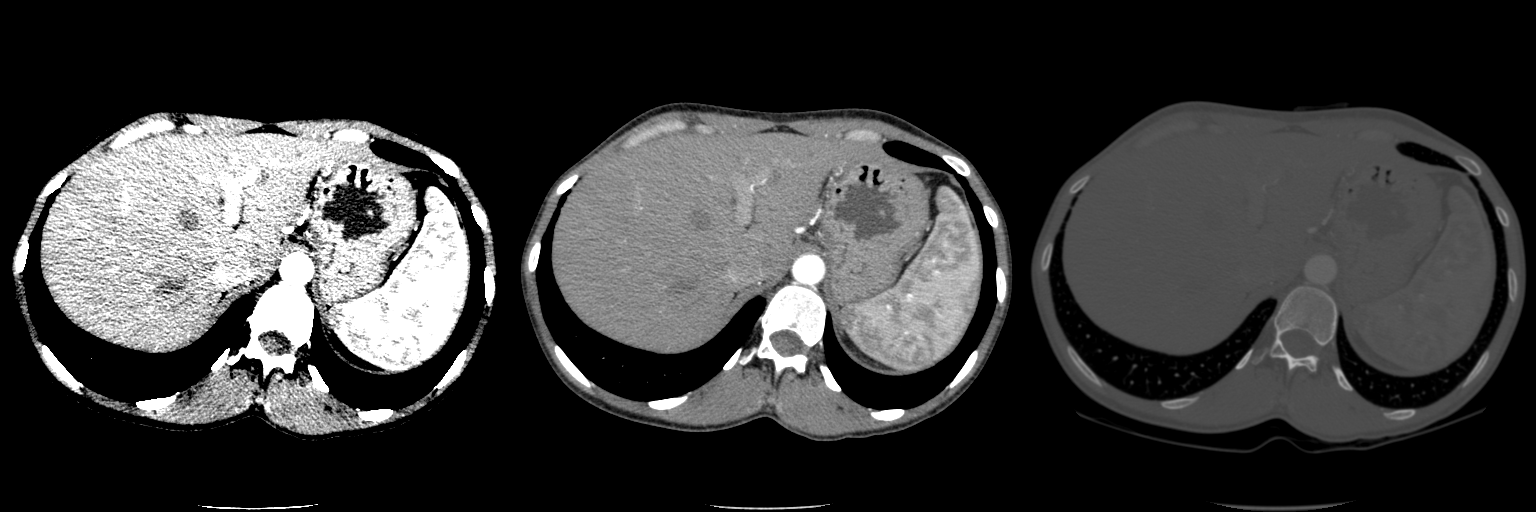
\includegraphics[width=\textwidth]{img/monochrome-002.png}
    \caption{Porównanie jednego obrazu w trzech różnych \enquote{funkcji okna}.}
    \label{fig:algorithm-pixmap-monochrome-multiwindow}
\end{figure}

\begin{figure}[!htbp]
    \centering
    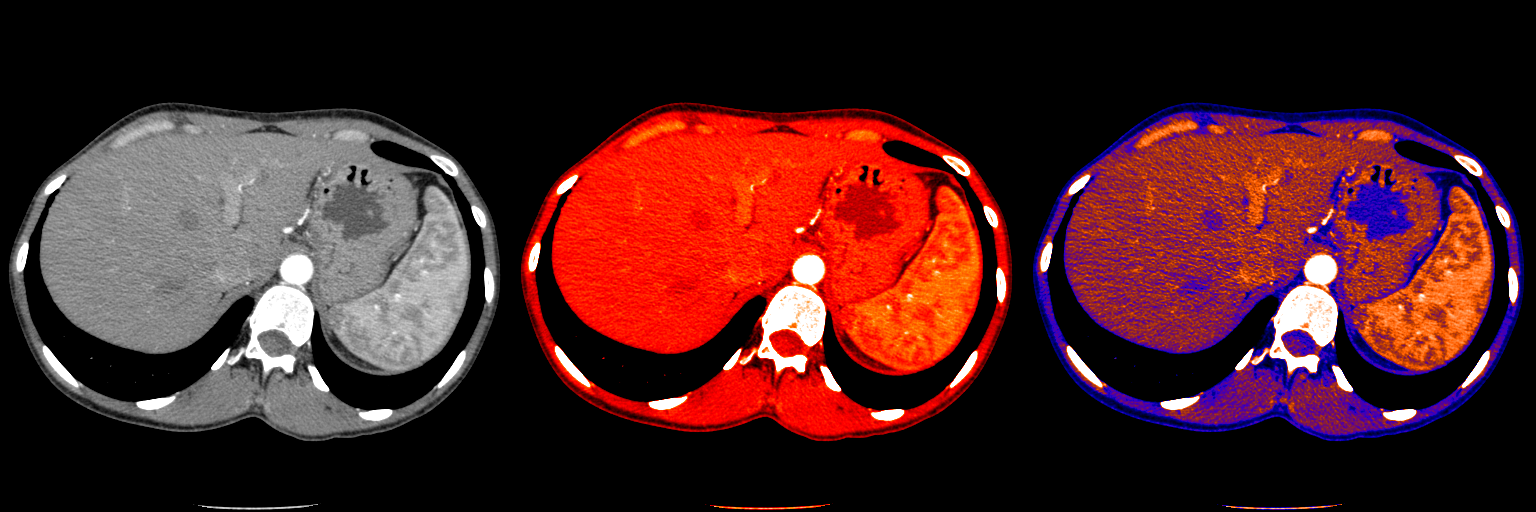
\includegraphics[width=\textwidth]{img/monochrome-003.png}
    \caption{Paleta Hot Iron (na środku) i Hot Metal Blue (po prawej) w porównaniu do palety w skali szarości (po lewej). Zdjęcie własne.}
    \label{fig:algorithm-pixmap-monochrome-palette}
\end{figure}


\subsubsection{Implementacja algorytmu}

\paragraph{Opis}
\par
Z uwagi na konieczność osiągnięcia dużej szybkości wyświetlania obrazu, warto jest szacować wartości funkcji f.
Wartości tej funkcji należy przeliczyć, gdy zmienione zostaną parametry tak zwanego \enquote{okna}.
Indeks koloru wyznaczany jest wtedy poprzez pobieranie wartości z tabeli o indeksie równym wartości numerycznej w obrazie.
Unikamy w ten sposób wielokrotnego wyznaczania wartości funkcji, która wymaga sprawdzenia warunku, czy dana wartość mieści się w wybranym przedziale wartości, w tak zwanym \enquote{oknie}, co jest bardzo kosztowne obliczeniowo.
Dlatego dobrym pomysłem jest stworzenie mniejszej tablicy typu LookUpTable, wypełnienie jej wszystkimi możliwymi wartościami obrazu, a następnie przerobienie obrazu z tablicą LUT.
Ponieważ tablica LUT posiada wszystkie możliwe kombinacje wartości, jej rozmiar można wyznaczyć wzorem: $2^N*3$, gdzie $N$ to liczba bitów liczby.
Standard \DICOM definiuje, że liczby mogą mieć $8$, $12$, $16$, $32$ i $64$ bity, jednakże, $12$ bitowe i tak się zapisuje w postaci 16-bitowych w pamięci RAM.
Dlatego możliwe wartości wielkości tablicy LUT to w przybliżeniu: $768$ bajtów, $196$ kilobajtów, $12,5$ gigabajtów i $56$ eksabajta ($55*10^{6}$ terabajtów).
Alokowanie dwóch największych wartości może być niemożliwe, dlatego w pracy wykonano dwie implementacje algorytmu: z tablicą LUT (dla 8 i 16 bitowych obrazów i bez tablicy LUT (dla 32 i 64 bitowych obrazów).
Algorytm składa się z 3 części: wyznaczenie parametrów \enquote{okna}, przygotowanie \enquote{okna} (tylko gdy jest tablica LUT), wielowątkowa iteracja po obrazie.
\par
Okno z LUT jest implementowane przez \sokarclass{Monochrome{\scopedots}WindowIntStatic}.
Okno bez LUT jest implementowane przez \sokarclass{Monochrome{\scopedots}WindowIntDynamic}.
Obie klasy dziedziczą po abstrakcyjnej klasie \sokarclass{Monochrome}{Window}, która z kolei dziedziczy po \sokarclass{SceneIndicator}, dlatego od razu może wyświetlać obecne wartości \enquote{okna}.
Decyzja o używanym \enquote{oknie} jest podejmowana podczas wczytywania obrazu przez klasę \sokarclass{Monochrome{\scopedots}Scene}
\par
UWAGA: Standard \DICOM zakłada, że danymi mogą być liczby całkowite(\cppcode{int}) oraz zmiennoprzecinkowe(\cppcode{float} lub \cppcode{double}), ale praktycznie, nie ma takich aparatów medycznych, które zapisywały by takie obrazy, gdzie dane to liczby zmiennoprzecinkowe.
Dlatego w pracy założono, że takie obrazy nie będą obsługiwane.

\paragraph{Wyznaczenie parametrów okna}
\par
Najpierw wyznaczam okienko, które zmienia wartości obrazu na skale od zera do jeden:
\[x_0 = center - width / 2\]
\[x_1 = center + width / 2\]
\[y_1 = 0.0\]
\[y_0 = 1.0\]
gdzie:
\begin{itemize}
    \item $center$ --- środek okienka
    \item $width$ --- szerokość okienka
    \item $x0$ i $y0$ --- współrzędne pierwszego punktu
    \item $x1$ i $y1$ --- współrzędne drugiego punktu
\end{itemize}
Przeglądarka pozwala na inwersje okienka.
Dlatego kiedy użytkownik zażyczy sobie inwersji, zmienne $y0$ i $y1$ zamienią się wartoścami.

Standard \DICOM przewiduje, że wszystkie dane powinny być wyskalowane, za pomocą wzoru.
\[OutputUnits = m*SV + b\]
gdzie:
\begin{itemize}
    \item $m$ --- wartość z \dicomtag{RescaleSlope}{0028}{1053}
    \item $b$ --- wartość z \dicomtag{RescaleIntercept}{0028}{1052}
    \item $SV$ --- stored values --- wartość woksela z pliku
    \item $OutputUnits$ --- wartość wynikowa
\end{itemize}

Wartości okienka odnoszą się do wartości już wyskalowanej, a ponieważ skalowanie całego obrazu jest czasochłonne, przeskalowanie okienka da taki sam efekt:
\[(OutputUnits - b ) / m = SV \]
więc:
\[x_0 -= rescaleIntercept\]
\[x_1 -= rescaleIntercept\]
\[x_0 /= rescaleSlope\]
\[x_1 /= rescaleSlope\]

Posiadamy, teraz dwa punkty okienka odnoszące się do wartości obrazu.
Wyznaczono parametry prostej przechodzącej przez dwa punkty:
\[a = (y_1 - y_0) / (x_1 - x_0)\]
\[b = y_1 - a * x_1\]

\par
Teraz algorytm się rozdwaja.
Pobieranie wartości z okienka odbywa się za pomocą funkcji \sokarclass{Monochrome}{Window\zerospace::{\zerospace}getPixel()}.

\paragraph{Implementacja dynamiczna bez tablicy LUT}

\par
W tej wersji funkcja \sokarfunction{Monochrome{\scopedots}Window}{getPixel} wygląda następująco:
\par
\begin{lstlisting}
inline const Pixel &getPixel(quint64 value) override {
    if (value < x0) {
        return background;
    } else if (value > x1) {
        return foreground;
    } else {
        return palette->getPixel(a * value + b);
    }
}
\end{lstlisting}
\par
Widzimy tutaj, że funkcja najpierw sprawdza czy zakres okienka został przekroczony, następnie wylicza wartość obrazu i pobiera kolor z palety.
\par
UWAGA: ponieważ nie istnieją rzeczywiste obrazy o wokselu 32-bitowym lub 64-bitowym, implementacja dynamiczna nie była testowana w warunkach rzeczywistych.

\paragraph{Implementacja statyczna z tablicą LUT}
\par
W wersji z LUT, podczas tworzenia okienka jest alokowany wektor obiektów \sokarclass{Pixel} klasy \stdclass{vector}{container/vector}.
Standard \DICOM przewiduje, że woksele mogą mieć wartości ujemne, więc tablica powinna mieć możliwość posiadania takich wartości indeksów, ale C++ nie przewiduje takiej możliwości.
Dlatego wprowadzono dwie zmienne pomocnicze \cppcode{maxValue} i \cppcode{signedMove}.
\cppcode{maxValue} jest to maksymalna wartość jaką dane mogą przyjąć, jest ona równa $2^N$, gdzie $N$ to liczba bitów brana z \dicomtag{BitsStored}{0028}{0101}.
A \cppcode{signedMove} to liczba przesunięcia liczb, przyjmuje wartość zero, gdy dane wokseli są całkowite nieujemne lub wartość przeciwną do \cppcode{maxValue}, gdy woksele są być ujemne.
Długość wektora pikseli jest sumą \cppcode{maxValue} i \cppcode{signedMove}.
A indeks woksela w wektorze ma wartość tego woksela zwiększoną o \cppcode{signedMove}.
\par
Wypełnienie wektora wartościami odbywa się poprzez iteracje po wszystkich możliwych wartościach, przeliczenie ich przez funkcje \enquote{okna}, a następnie wstawienie ich do wektora.
W celu poprawy szybkości, zastosowano sprawdzanie czy wartości są w zakresie \enquote{okna}.
Poniżej kod funkcji:
\begin{lstlisting}
bool genLUT() override {

    if (WindowInt::genLUT()) {

        /* Przeskalowanie wektora, gdy jest to wymagane */
        if (arraySize != signedMove + maxValue) {
            arraySize = signedMove + maxValue;
            arrayVector.resize(arraySize);
        }

        /* Wyliczenie najmniejszej wartości */
        qreal x = qreal(signedMove) * -1;

        auto &background = isInversed() ? palette->getForeground() : palette->getBackground();
        auto &foreground = isInversed() ? palette->getBackground() : palette->getForeground();

        /* Iteracja */
        pixelArray = &arrayVector[0];
        for (int i = 0; i <= arraySize; i++) {

            if (x < x0) {
                *pixelArray = background;
            } else if (x > x1) {
                *pixelArray = foreground;
            } else {
                *pixelArray = palette->getPixel(a * x + b);
            }

            x++;
            pixelArray++;
        }

        pixelArray = &arrayVector[0];

        updateLastChange();

        return true;
    }
    return false;
}
\end{lstlisting}

\par
Funkcja zmiany wartości obrazu na kolor prezentuje się następująco:
\begin{lstlisting}
inline const Pixel &getPixel(quint64 value) override {
    return *(pixelArray + signedMove + value);
}
\end{lstlisting}

\paragraph{Iterowanie po obrazie}
\par
Po wygenerowania obrazu, należy przeiterować go przez funkcje \enquote{okna}.
Do zokienkowania jednego piksela nie potrzeba innego piksela dlatego w celu przyspieszenia procesu okienkowania, iteracja po obrazie odbywa się w wielu wątkach.
\par
W C++ typy zmiennych muszą być zdefiniowane przed kompilacją, co jest bardzo problematyczne.
Mając dwa typy okienek, każde odsługujące 4 typy liczb całkowitych, musiało by zostać zaimplementowanych 8 prawie identycznych funkcji.
Dlatego podział ten został zaimplementowany za pomocą 4 funkcji z szablonami:
\begin{itemize}
    \item \sokarfunction{Monochrome{\scopedots}Scene}{genQPixmapOfTypeWidthWindowThread}

          Jest funkcją jednego wątku, który iteruje po obrazie.
          Jego parametrami są zakresy podane w indeksach wokseli po któych ma iterować.
          \cppcode{IntType} to jest typ zmiennej woksela obrazu.
          \cppcode{WinClass} klasa okienka.
          Nazewnictwo będzie kontynuowane w następnych punktach.
          Kod funkcji:
          \begin{lstlisting}
template<typename IntType, typename WinClass>
void Monochrome::Scene::genQPixmapOfTypeWidthWindowThread(quint64 from, quint64 to) {

    auto buffer = &targetBuffer[from];
    auto origin = (IntType *) &originBuffer[0];
    auto windowPtr = (WinClass *) getCurrentWindow();

    origin += from;

    for (quint64 i = from; i < to; i++, origin++) {
        /* W tym miejscu jest dokonywana zamiana liczby na kolor */
        *buffer++ = windowPtr->getPixel(*origin);
    }
}
\end{lstlisting}

    \item \sokarfunction{Monochrome{\scopedots}Scene}{genQPixmapOfTypeWidthWindow}

          Jest to funkcja, która dzieli obraz na wątki, tworzy je i uruchamia.
          Ilość wątków jest ustalana za pomocą funkcji \qtfunction{QThread}{idealThreadCount}.
          Wątki działają na zakresach o długości ilości wokseli podzielonej przez ilość wątków.
          Kod funkcji:
          \begin{lstlisting}
template<typename IntType, typename WinClass>
void Monochrome::Scene::genQPixmapOfTypeWidthWindow() {

    /* Tworzenie wektora wątków */
    std::vector<std::thread> threads;

    quint64 max = imgDimX * imgDimY;
    quint64 step = max / QThread::idealThreadCount();

    for (int i = 1; i < QThread::idealThreadCount(); i++) {
        std::thread t(&Scene::genQPixmapOfTypeWidthWindowThread<IntType, WinClass>,
                      this,
                      i * step,
                      std::min((i + 1) * step, max));

        threads.push_back(std::move(t));
    }

    /* W celu zmniejszenia ilości wątków, wątek obecny też zostanie wykorzystany */
    genQPixmapOfTypeWidthWindowThread<IntType, WinClass>(0, step);

    /* Czekanie na wszystkie wątki */
    for (auto &t: threads) t.join();
}
\end{lstlisting}

    \item \sokarfunction{Monochrome{\scopedots}Scene}{genQPixmapOfType}

          Jest to funkcja pomocnicza ustalająca obecną klasę obecnego \enquote{okna}, aby móc wykonać funkcje \sokarfunction{Monochrome{\scopedots}Scene}{genQPixmapOfTypeWidthWindow}.
          Kod funkcji:
          \begin{lstlisting}
template<typename IntType>
void Monochrome::Scene::genQPixmapOfType() {

    switch (getCurrentWindow()->type()) {
        case Window::IntDynamic:
            genQPixmapOfTypeWidthWindow<IntType, WindowIntDynamic>();
            break;

        case Window::IntStatic:
            genQPixmapOfTypeWidthWindow<IntType, WindowIntStatic>();
            break;

        default:
            throw WrongScopeException(__FILE__, __LINE__);
    }
}
\end{lstlisting}

    \item \sokarfunction{Monochrome{\scopedots}Scene}{generatePixmap}

          Funkcja odświeża okienko i sprawdza, czy odświeżenie obrazu jest konieczne, następnie sprawdza typ liczby woksela i uruchamia \sokarfunction{Monochrome{\scopedots}Scene}{genQPixmapOfType}.
          Kod funkcji:
          \begin{lstlisting}
bool Monochrome::Scene::generatePixmap() {

    /* Odświeżamy okno i sprawdzamy czy odświeżenie obrazu jest konieczne */
    getCurrentWindow()->genLUT();
    if (lastPixmapChange >= getCurrentWindow()->getLastChange()) return false;

    /* Sprawdzamy typ liczby woksela obrazu */
    switch (gdcmImage.GetPixelFormat()) {
        case gdcm::PixelFormat::INT8:
            genQPixmapOfType<qint8>();
            break;
        case gdcm::PixelFormat::UINT8:
            genQPixmapOfType<quint8>();
            break;
        case gdcm::PixelFormat::INT16:
            genQPixmapOfType<qint16>();
            break;
        case gdcm::PixelFormat::UINT16:
            genQPixmapOfType<quint16>();
            break;
        case gdcm::PixelFormat::INT32:
            genQPixmapOfType<qint32>();
            break;
        case gdcm::PixelFormat::UINT32:
            genQPixmapOfType<quint32>();
            break;
        case gdcm::PixelFormat::INT64:
            genQPixmapOfType<qint64>();
            break;
        case gdcm::PixelFormat::UINT64:
            genQPixmapOfType<quint64>();
            break;

        default: /* W przypadku innych jest zwracany wyjątek */
            throw Sokar::ImageTypeNotSupportedException();
    }

    pixmap.convertFromImage(qImage);
    return true;
}
\end{lstlisting}
\end{itemize}

\subsubsection{Palety}
Klasa \sokarclass{Palette} reprezentuje palety kolorów używanych do pseudokolorwania obrazu.
Paleta przerabia liczbę zmiennoprzecinkową od zera do jedynki na kolor RGB, zwracając \sokarclass{Pixel}.
Paleta nie ma zdefiniowanej długości minimalnej i maksymalnej.

\par
Palety są wczytywane z plików XML w czasie uruchamiania programu i można definiować własne palety nie będące częścią standardu.
Przykładowy wygląd pliku palety HotIron:
\begin{lstlisting}[language=XML]
<palette display="Hot Iron" name="HOT_IRON">

    <entry red="0" green="0" blue="0"/>
    <entry red="2" green="0" blue="0"/>
    <entry red="4" green="0" blue="0"/>

    ...

    <entry red="254" green="0" blue="0"/>
    <entry red="255" green="0" blue="0"/>
    <entry red="255" green="2" blue="0"/>

    ...

    <entry red="255" green="250" blue="248"/>
    <entry red="255" green="252" blue="252"/>
    <entry red="255" green="255" blue="255"/>
</palette>
\end{lstlisting}

\subsection{Tworzenie transformat i ich użycie na obrazie}
\label{sec:algorithm-pixmap-tranformat}

\par
Wygenerowany obraz można wyświetlić na scenie bez większego problemu.
Wyświetlanie \cppcode{pixmap}, obiektu klasy \qtclass{QPixmap}, odbywa się za pomocą obiektu \cppcode{pixmapItem}, obiektu klasy \qtclass{QGraphicsPixmapItem}, który dziedziczy po \qtclass{QGraphicsItem}.
Ta ostatnia klasa ma w sobie zaimplementowaną funkcję pozwalającą na nałożenie przekształcenia na obraz.
Transformata to obiekt klasy \qtclass{QTransform}, który reprezentuje transformatę dwu wymiarowa na obiekt, praktycznie jest to macierz 3 na 3 reprezentująca przekształcenie w współrzędnych jednorodnych.
\par

Zostało zdefiniowanych 4 transformat:
\begin{itemize}
    \item \cppcode{centerTransform} --- transformata wyśrodkowująca, zadanie tego przekształcenia jest przeniesienie obrazu na środek sceny
    \item \cppcode{panTransform} --- transformata przesunięcia
    \item \cppcode{scaleTransform} --- transformata skali
    \item \cppcode{rotateTransform} --- transformata rotacji
\end{itemize}

Te cztery transformaty są łączone za pomocą wirtualnej funkcji \sokarfunction{DicomScene}{getPixmapTransformation}.
Kod funkcji:
\begin{lstlisting}
QTransform DicomScene::getPixmapTransformation() {
	QTransform transform;
	transform *= centerTransform;
	transform *= scaleTransform;
	transform *= rotateTransform;
	transform *= panTransform;
	return transform;
}
\end{lstlisting}
\qtclass{QTransform} posiada operator mnożenie, dlatego można mnożyć obiekty tej klasy jak liczby.
Realizuje on takie równanie:
\[panTransform*rotateTransform*scaleTransform*centerTransform\]

\subsubsection{Współrzędne jednorodne}

Współrzędne jednorodne definiuje się jako sposób reprezentacji punktów n-wymiarowej przestrzeni rzutowej za pomocą układu $n+1$ współrzędnych.
W bibliotece Qt jedną z implementacji współrzędnych jednorodnych jest klasa \qtclass{QTransform}.
Implementuje ona podstawowe zachowania macierzy 3 na 3 jak również wbudowane operacje takie jak: przesuwanie implementowane prze \qtfunction{QTransform}{translate}, obrót implementowany przez funkcje \qtfunction{QTransform}{rotate} i skalowanie implementowane przez \qtfunction{QTransform}{scale}.

Przykład działania:
\begin{lstlisting}
QTransform transform;
transform.translate(50, 50);
transform.rotate(45);
transform.scale(0.5, 1.0);
\end{lstlisting}
Powyższa transformata skaluje obiekt na 50\% szerokości, obraca o 45 stopni, przesuwa o 50 punktów na osi $x$ i $y$.

\par
Taką transformatę można nałożyć na obiekty klasy \qtclass{QGraphicsPixmapItem}.

\subsubsection{Interakcja z użytkownikiem}

Trzy transformaty (bez wyśrodkowującej) są zmieniane w trakcie interakcji z użytkownikiem.
Są zmieniane w dwóch przypadkach: po odebraniu sygnału od paska zadań, obiektu klasy \sokarclass{DicomToolbar} lub podczas ruchu myszki, gdy wciśnięty jest prawy przycisk.

\paragraph{Zmiany poprzez oderanie sygnału}

\par
Na pasku zadań, nad sceną, znajduje się szereg przycisków, które po wciśnięciu wysyłają sygnał do obecnej sceny poprzez obiekt klasy \sokarclass{DicomView}.
Sposób wysyłania sygnałów jest szerzej opisany w sekcji \ref{sec:sokar-dicomtoolbar}.

\par
Po otrzymaniu odpowiedniego sygnału jest wykonywana operacja na transformacie.
Wszystkie transformaty są implementowane przez wirtualną funkcje \sokarfunction{DicomScene}{toolBarActionSlot}, która jest slotem.

\par
Lista opisów reakcji na sygnały (stan zerowy transformaty, to stan w którym transformata nic nie robi):
\begin{itemize}

    \item \cppcode{ClearPan} --- przywraca transformatę przesunięcia do stanu zerowego

    \item \cppcode{Fit2Screen} --- przywraca transformatę skali do stanu zerowego, następnie wylicza nową skalę w zależności od wymiarów obrazu i sceny

    \item \cppcode{OriginalResolution} --- przywraca transformatę skali do stanu zerowego

    \item \cppcode{RotateRight90} --- na transformacie rotacji zostaje użyta funkcja \qtfunction{QTransform}{rotate} z parametrem $90$.

    \item \cppcode{RotateLeft90} --- na transformacie rotacji zostaje użyta funkcja \qtfunction{QTransform}{rotate} z parametrem $-90$.

    \item \cppcode{FlipHorizontal} --- na transformacie rotacji zostaje użyta funkcja \qtfunction{QTransform}{scale} z parametrami $1$ i $-1$.

    \item \cppcode{FlipVertical} --- na transformacie rotacji zostaje użyta funkcja \qtfunction{QTransform}{scale} z parametrami $-1$ i $1$.

    \item \cppcode{ClearRotate} --- przywraca rotacji do stanu zerowego

\end{itemize}
Oczywiście po zmianie transformaty jest wywoływana funkcja \sokarfunction{DicomScene}{updatePixmapTransformation}, która odświeża transformatę na obiekcie \cppcode{pixmapItem}.

\paragraph{Zmiany poprzez obsługę myszki}

\par
\qtclass{QGraphicsScene} dostarcza możliwość obsługi myszki poprzez wirtualną funkcje \qtfunction{QGraphicsScene}{mouseMoveEvent}.
Dzięki temu obsługa myszki może być rozszerzana przez wszystkie klasy dziedziczące po tej klasie.
Dodatkowo funkcja ta dostarcza obiekt klasy \qtclass{QGraphicsSceneMouseEvent}, w którym znajdują się informacje o pozycji myszki jak i ostatniej pozycji myszki.

\par
Jeżeli jest wykryty ruch myszki z wciśniętym lewym przyciskiem myszy, to w zależności od stanu paska narzędzi, wywoływana jest odpowiednia akcja.
Akcje są obsługiwane przez klasy \sokarclass{DicomScene} i \sokarclass{Monochrome{\scopedots}Scene}.
Każda z nich obsługuje pewną pule stanów.
Lista obsługiwanych stanów paska narzędzi:
\begin{itemize}
    \item \cppcode{Pan} --- stan przesuwania, obsługiwany przez \sokarclass{DicomScene}

          Na transformacie przesuwania jest wywoływana jest funkcja przesunięcia \qtfunction{QTransform}{translate} z parametrami odpowiadającymi przesunięciu myszki.

    \item \cppcode{Zoom} --- stan skalowania, obsługiwany przez \sokarclass{DicomScene}

          Na transformacie skalowania jest wywoływana jest funkcja skalowania \qtfunction{QTransform}{scale} z parametrem \cppcode{scale} wyliczanym podanym wzorem:

          \[scale=1\]
          \[scale=scale-{\Delta}y*0.01\]
          \[scale=scale-{\Delta}x*0.001\]

          Sprawia to, że ruch pionowy jest bardzie czuły na zmianę niż ruch poziomy.
          Teoretycznie jest możliwość implementacji odrębnego skalowania w dwóch osiach, jednakże jest to nie intuicyjne w wprowadza użytkownika w zakłopotanie.

    \item \cppcode{Rotate} --- stan rotacji, obsługiwany przez \sokarclass{DicomScene}

          Na transformacie rotacji jest wywoływana jest funkcja rotacji \qtfunction{QTransform}{rotate} z parametrem \cppcode{rotate} wyliczanym podanym wzorem:

          \[rotate = 0\]
          \[rotate = rotate + {\Delta}y * 0.5;\]
          \[rotate = rotate + {\Delta}x * 0.1;\]

          Sprawia to, że ruch pionowy jest bardzie czuły na zmianę niż ruch poziomy.

    \item \cppcode{Windowing} --- stan okienkowania, obsługiwany przez \sokarclass{Monochrome{\scopedots}Scene}

          Do obiektu okienka są wysyłane zmiany poprzez funkcje: \sokarfunction{Window}{mvVertical} z parametrem ${\Delta}y$ i \sokarfunction{Window}{mvHorizontal} z parametrem ${\Delta}x$
          Następnie ponownie jest generowany obraz z uwzględnieniem zmiany okienka.

\end{itemize}

\subsection{Ustalanie pozycji pacjenta względem sceny}
\label{sec:algorithm-imageorientationindicator}

W obrazie \DICOM jest pośrednio zapisana informacja o ułożeniu obrazu względem pacjenta.
Celem algorytmu jest określenie jaką pozycje przyjmuje pacjent w stosunku do sceny, tak aby można było wyświetlić ta pozycje na scenie.

\subsubsection{Format zapisu informacji o orientacji obrazu}

\par
Informacje o orientacji oraz pozycji względem pacjenta znajdują się w odpowiednio w tagach \dicomtag{ImageOrientation}{0020}{0037} i \dicomtag{ImagePosition}{0020}{0032}.

\par
Standard \DICOM zdefiniował ułożenie osi we współrzędnych kartezjańskich następująco:
\begin{itemize}
    \item \quotett{x} --- oś przechodząca od prawej do lewej strony pacjenta, \dataword{L} oznacza zwrot zgodny z osią, a \dataword{R} oznacza zwrot przeciwny

    \item \quotett{y} --- oś przechodząca od przodu do tyłu pacjenta, \dataword{P} oznacza zwrot zgodny z osią, a \dataword{A} oznacza zwrot przeciwny

    \item \quotett{z} --- oś przechodząca od dołu do góry pacjenta, \dataword{H} oznacza zwrot zgodny z osią, a \dataword{F} oznacza zwrot przeciwny

\end{itemize}

\begin{figure}[!htbp]
    \centering
    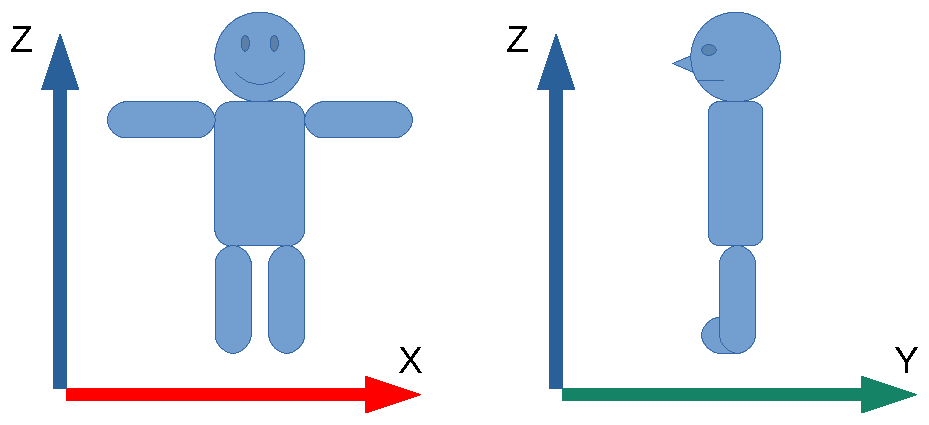
\includegraphics[width=0.7\textwidth]{img/imageorientationindicator-003.pdf}
    \caption{Wizualizacja układu osi współrzędnych kartezjańskich pacjenta. Zdjęcie własne.}
    \label{fig:imageorientationindicator2}
\end{figure}

\par
Wartość \dicomtag{ImageOrientation}{0020}{0037} składa się z sześciu liczb, opowiednio oznaczanych dalej X\textsubscript{x}, X\textsubscript{y}, X\textsubscript{z}, Y\textsubscript{x}, Y\textsubscript{y}, Y\textsubscript{z}.
Standard DICOM definiuje, że te dane mają być z interpretowane w następujący sposób:
\[
    \begin{bmatrix}
        P_x \\ P_y \\ P_z \\ 1
    \end{bmatrix}
    =
    \begin{bmatrix}
        X_x\Delta_i & Y_x\Delta_j & 0 & S_x \\
        X_y\Delta_i & Y_y\Delta_j & 0 & S_y \\
        X_z\Delta_i & Y_z\Delta_j & 0 & S_z \\
        0           & 0           & 0 & 1
    \end{bmatrix}
    \begin{bmatrix}
        i \\ j \\ 0 \\ 1
    \end{bmatrix}
    =
    M
    \begin{bmatrix}
        i \\ j \\ 0 \\ 1
    \end{bmatrix}
\]
gdzie:
\begin{itemize}
    \item $P_{xyz}$ --- koordynaty woksela (i,j) w współrzędnych obrazu wyrażone w milimetrach
    \item $S_{xyz}$ --- trzy wartości z elementu ze znacznikiem \dicomtag{ImagePosition}{0020}{0032}. Oznacza punkt pozycji pacjenta wyrażony w milimetrach w stosunku do urządzenia wykonującego pomiar.
    \item $X_{xyz}$ --- trzy pierwsze wartości z \dicomtag{ImageOrientation}{0020}{0037}
    \item $Y_{xyz}$ --- trzy ostatnie wartości z \dicomtag{ImageOrientation}{0020}{0037}
    \item $i$ i $j$ --- oznaczają współrzędne na macierzy obrazu, odpowiednio kolumnę i wiersz. Zero oznacza początek.
    \item $\Delta_i$ i $\Delta_j$ --- rzeczywista wielkość piksela obrazu wyrażoną w milimetrach, w algorytmie wyznaczania strony pacjenta ta wartość, może wynosić 1, ponieważ odpowiada za skale
\end{itemize}

Praktycznie rzecz biorąc, pierwsza macierz to wektor reprezentujący pozycję pacjenta.
Druga jest to transformata.
Trzecia to pozycja na obrazie.

\subsubsection{Wyznaczanie pozycji pacjenta}

Interesuje nas wyznaczenie pozycji sześciu (punktów) na płaszczyźnie obrazu.
Załóżmy, że pacjent znajduje się w środku układu współżędnych i jest nieskończenie mały.
Możemy więc zdefiniować sześć punktów o następujących współrzędnych, dalej używanych pod nazwą $PatientPosition$, które będą odpowiadały stroną pacjenta:
\begin{itemize}
    \item \quotett{R} - $[-1, 0, 0, 1]$
    \item \quotett{L} - $[+1, 0, 0, 1]$
    \item \quotett{A} - $[0, -1, 0, 1]$
    \item \quotett{P} - $[0, +1, 0, 1]$
    \item \quotett{F} - $[0, 0, -1, 1]$
    \item \quotett{H} - $[0, 0, +1, 1]$
\end{itemize}
Punkty $PatientPosition$ odpowiadają punktom $P_{xyz}$ z równania ze standardu \DICOM.

\par
UWAGA: Wszystkie obliczenia odbywają się w współrzędnych jednorodnych.

\par
Na równaniu z poprzedniego punktu wykonuje takie przekształcenie:
\[PatientPosition = imgMatrix * ScenePosition\]
\[imgMatrix^{-1} * PatientPosition = imgMatrix^{-1} * imgMatrix * ScenePosition\]
\[imgMatrix^{-1} * PatientPosition = ScenePosition\]
\[ScenePosition = imgMatrix^{-1} * PatientPosition\]
gdzie:
\begin{itemize}
    \item $imgMatrix$ --- macierz przekształcenia obrazu, o której będzie dalej
    \item $ScenePosition$ --- pozycja na obrazie, która naz interesuje
    \item $PatientPosition$ --- któryś z punktów względem pacjenta.
\end{itemize}
\par
Wygląd macierzy $imgMatrix$:
\[
    \begin{bmatrix}
        X_x & Y_x & 0 & 0 \\
        X_y & Y_y & 0 & 0 \\
        X_z & Y_z & 0 & 0 \\
        0   & 0   & 0 & 1
    \end{bmatrix}
\]
Powyższa macierz różni się od macierzy definiowanej w standardzie.
Po pierwsze PikselSpacing został pominięty, a konkretniej nadałem mu wartość 1.
Po drugie pozycja z \dicomtag{ImagePosition}{0020}{0032} została zrównana do punktu zerowego, dzięki temu, wynik też będzie względem punktu zero.
Wyznaczenie macierzy $imgMatrix$ jest jednorazowe.

\par
Po wyznaczeniu sześciu punktów $ScenePosition$, po jednej dla każdego punktu względem pacjenta są zapisywane. $ScenePosition$ odpowiada pozycji punktów na obrazie w pozycji startowej.

\par
Na scenie, której jest wyświetlany obraz, użytkownik, może obracać obraz o dowolny kąt, według własnego uznania.
Te przekształcenia, są realizowane za pomocą macierzy rotacji, dalej znana jako $rotateTransform$.
Macierz $rotateTransform$ jest przesyłana do naszego obiektu \sokarclass{ImageOrientationIndicator} za każdym razem kiedy zostanie zmieniona.

\par
Ostateczne wyznaczenie pozycji punktów pacjent na obrazie odbywa sie przez przemnożenie lewostronne $rotateTransform$ i $ScenePosition$.
\[rotateTransform * ScenePosition\]
Wyznaczane jest w ten sposób pozycja sześciu punktów pacjenta na płaszczyźnie sceny wyświetlanej.
Następnie określane jest na, której z ośmiu części płaszczyzny jest umieszczony dany punkt, podział płaszczyzny jest widoczny na rysunku \ref{fig:imageorientationindicator4}.
Tej płaszczyźnie nadawany jest tytuł w postaci litery, która oznacza stronę pacjenta.
Jeżeli punkt znajduje się w centrum, na przecięciu osi, to oznacza, że punkt znajduje się za lub przed ekranem, więc jest pomijany.
Następnie do czterech pól wyświetlających zostają wstawione następujące teksty:
\begin{itemize}
    \item lewe pole: tytuł części 7, tytuł części 0 i tytuł części 1
    \item górne pole: tytuł części 1, tytuł części 2 i tytuł części 3
    \item prawe pole: tytuł części 3, tytuł części 4 i tytuł części 5
    \item dolne pole: tytuł części 7, tytuł części 6 i tytuł części 5
\end{itemize}

\par
Przykład:\\
Punkt \quotett{H}, czyli punkt reprezentujący kierunek głowy, został przypisany do części 1 i odpowiednio \quotett{L} do części 7, \quotett{R} do części 3 i \quotett{F} do części 5.
Punkty \quotett{A} i \quotett{P} zostały pominięte ponieważ znalazły się na środku.
Do lewego pola wstawiany jest tekst \quotett{HL}, do górnego \quotett{HR}, do prawego \quotett{RF} i do dolnego \quotett{LF}.

\begin{figure}[!htbp]
    \centering
    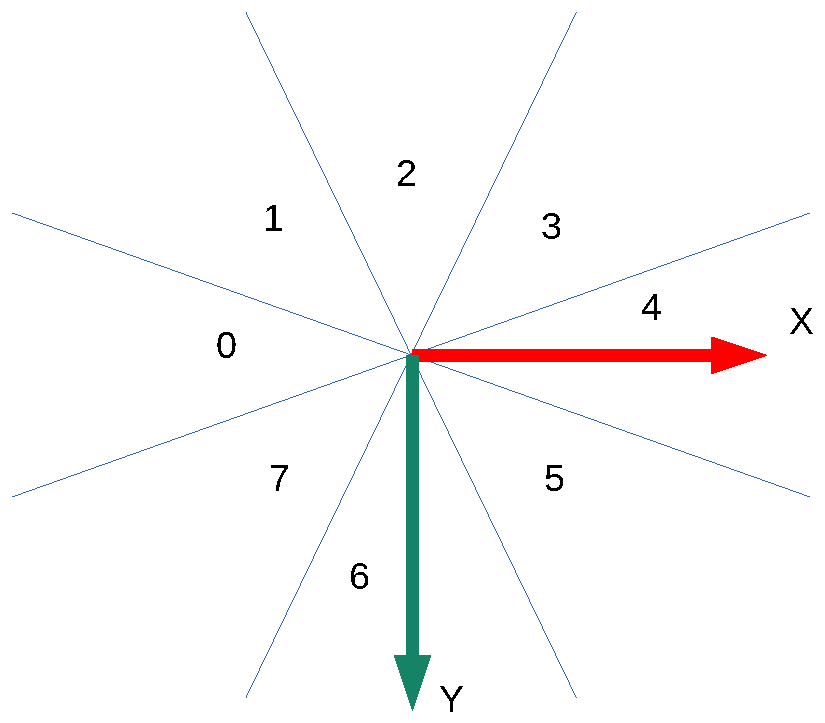
\includegraphics[width=0.5\textwidth]{img/imageorientationindicator-004.pdf}
    \caption{Podział płaszczyzny sceny. Wyróżniono osiem części. Zdjęcie własne.} 
    \label{fig:imageorientationindicator4}
\end{figure}

\par
Przykład można zobaczyć na rysunku \ref{fig:imageorientationindicator1}.
Na obrazie widzimy, że lewa strona pacjenta znajduje się po prawej stronie obrazu, prawa strona pacjenta po lewej, góra pacjenta na górnej części obrazu.
Wynika z tego, że obraz przedstawia pacjenta skierowanego twarzą do nas.

\begin{figure}[!htbp]
    \centering
    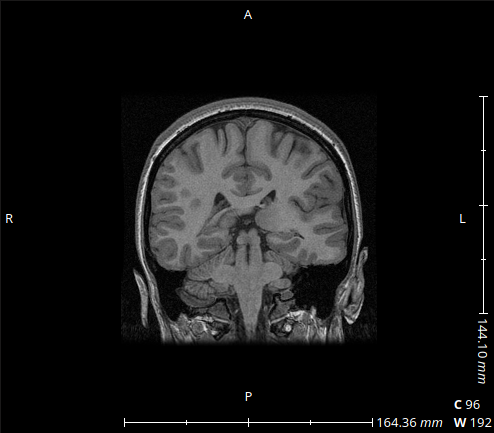
\includegraphics[width=100mm]{img/imageorientationindicator-002.png}
    \caption{Przykładowy obraz medyczny (przekrój głowy MR) z oznaczeniem orientacji obrazu z apomocą liter A, P, R, L, F, H. Zdjęcie własne.}
    \label{fig:imageorientationindicator1}
\end{figure}


\section{Konwertowanie i analiza danych w tagach}

Każdy plik DICOM posiada \quotett{Data Set}, czyli zbiór informacji składający się z \quotett{Data Element}.
\quotett{Data Element} jest strukturą przechowującą wszystkie dane dotyczące obrazu.

\paragraph{Budowa \textquote{Data Element}}

\begin{itemize}
    \item Data Element Tag - to unikalny identyfikator, złożony z dwóch liczb: grupy(uint16) i elementu(uint16) grupy.
    Obiekt używany do przechowywania taga to \gdcmclass{Tag}.
    Informuje o znaczeniu danych.
    Na przykład: jeżeli tag przyjmie wartość \dicomtag{PatientName}{0010}{0010}, oznacza to, że dane w \textquote{Data Element} zawierają nazwę pacjenta.
    \item Value Representation, w skrócie VR – typ danych umożliwiający poprawną interpretację danych.
    Informuje w jaki sposób dane są zapisane.
    Obiekt używany do przechowywania taga to \gdcmclass{VR}.
    Na przykład: Decimal String, w skrócie DS, oznacza liczbę zapisaną za pomocą teksu.
    Czasami to pole może być puste, wtedy należy się odnieść do VR przypisanego do taga, który określa standard.
    \item Value Length, w skrócie VL – rozmiar elementu
    \item Value Field (opcjonalne) – pole z właściwymi danymi
\end{itemize}

\paragraph{Konwerter}

Obiekt klasy \sokarclass{DataConverter} to obiekt zajmujący się konwersją danych z pliku DICOM na dane w formacie odpowiadającej przeglądarce.

Kilka rzeczy które się tyczą wszystkich danych i konwersji:
\begin{itemize}
    \item większość VR jest to zapisane jako tekst, kodowanie i dekodowanie tekstu jest zapewniane przez bibliotekę, a konkretniej przez klasę \gdcmclass{StringFilter}, dlatego nie przejmuje się takimi rzeczami jak zapisem LittleEndian i BigEndian.
    \item większość danych może mieć kilka wartości oddzielonych backslashem \quotett{\textbackslash}, dlatego konwerter dla VR w, których standard przewiduje wiele wartości, zawsze zwraca \qtclass{QVector} z tymi wartościami
    \item wszystkie dane są zapisane parzystą ilością bajtów, w przypadku tekstu dodaje się znak spacji na końcu danych, taka spacja jest pomijana w analizie danych
\end{itemize}

Klasa obsługuje następujące VR:
\begin{itemize}
    \item AS - Age String - wiek lub długość życia

    Długość danych zawsze wynosi 4 bajty.
    Pierwsze trzy bajty to liczba całkowita zapisana za pomocą tekstu.
    Czwarty bajt to znaku określający jednostkę czasu.
    Standard definiuje cztery możliwe jednostki czasu: \quotett{D} jako dzień, \quotett{W} jako tydzień, \quotett{M} jako miesiąc, oraz \quotett{Y} jako jeden rok.
    Konwerter zmienia tą wartość na tekst w postaci czytelnej, np: \quotett{18 weeks} lub \quotett{3 years}, oraz jest wrażliwy na obecny język aplikacji.
    
    Przykład: \quotett{018M} oznacza 18 miesięcy, \quotett{123D} oznacza 123 dni.

    \item AT - Attribute Tag - inny tag

    Długość danych to zawsze 32 bity, są to dwie 16 bitowe liczby.
    Odpowiednio grupa i element grupy.
    Ten VR jest używany kiedy wskazujemy na inny tag.
    Wartość nie jest nigdy pokazywana użytkownikowi, a jedynie używana w interpretacji przez algotyrm tworzenia filmu.
    
    Przykład: tag \dicomtag{FrameIncrementPointer}{0028}{0009} jest używany kiedy w pliku jest zapisana sekwencja kilku obrazów, wskazuje on na inny tag zawierający informacje w jaki sposób ta sekwencja ma być wyświetlona.
    
    \item DA - Date - data lub dzień

    Długość danych zawsze wynosi 8 bajtów.
    Data zapisana w formacie \quotett{YYYYMMDD}, gdzie: \quotett{YYYY} cztery cyfry roku, \quotett{MM} dwie cyfry miesiąca, \quotett{DD} dwie cyfry dnia w kalendarzu Gregoriańskim.
    Konwerter zamienia dane na obiekt klasy \qtclass{QDate}, który ma w sobie wbudowaną konwersję na tekst zależny od ustawień językowych aplikacji.
    
    Przykład: \quotett{19800716} oznacza 16 lipca 1980
    
    UWAGA: Standard \quotett{ACR-NEMA Standard 300}, czyli poprzednik DICOM definiował date w sposób \quotett{YYYY.MM.DD}, według standardu DICOM, taki zapis jest nie poprawny, ale zdarzają się stare obrazy z takimi datami i \sokarclass{DataConverter} obsługuje taki format.

    \item DS - Decimal String - liczba zmienno przecinkowa lub ciąg kilku liczb zmienno przecinkowych zapisanych za pomocą tekstu w notacji wykładniczej

    Długość jednej liczby powinna maksymalne wynosić 16 bajtów.
    Dostępne znaki to \quotett{0}-\quotett{9}, \quotett{+}, \quotett{-}, \quotett{E}, \quotett{e}, \quotett{.}.
    Biblioteka QT posiada wbudowany konwerter liczb zapisanych w formacie wykładniczym, dlatego mój konwerter dzieli tekst i konwertuje za pomocą QT.
    
    Przykład: \quotett{426\textbackslash468 } oznacza dwie liczby 426 i 468. Proszę zwrócić uwagę na spacje na końcu.

    \item IS - Integer String - liczba całkowita 

    Długość jednej liczby powinna maksymalne wynosić 12 bajtów.
    Dostępne znaki to \quotett{0}-\quotett{9}, \quotett{+}, \quotett{-}.
    Biblioteka QT posiada wbudowany konwerter liczb całkowitych, dlatego mój konwerter używa konwertera z QT.
    
    Przykład: \quotett{426 }  oznacza liczbę 426.

    \item PN - Person Name - nazwa osoby

    Jako, że pacjenta, bądź obiekt badany można nazwać w sposób dowolny i odbiegający od polskiego standardu nazewnictwa, standard DICOM nie przewiduje rozdzielenie poszczególnych składowych nazwy na oznaczone fragmenty.
    \quotett{Person Name} dzieli nazwę na podane fragmenty, rozdzielony znakiem \quotett{\^{}} (94 znak kodu ASCII):
    \begin{itemize}
        \item family name complex - nazwisko, np. Smolik
        \item given name complex - imię, np. Adam
        \item middle name - środkowe imię, brak odpowiednika w polskim nazewnictwie
        \item name prefix - prefiks przed imieniem, np: mgr. inż.
        \item name suffix - sufiks po imieniu, brak odpowiednika
    \end{itemize}
    Długość jednego fragmenty powinna maksymalne wynosić 64 znaki.
    W przypadku mniejszej ilości segmentów, mamy założyć, że są puste.
    
    Przykład: \quotett{prof. dr. hab. inż. Waldemar Smolik pracownik ZEJIM} był by zapisany w sposób następujący: \quotett{Smolik\^{}Waldemar\^{}\^{}prof. dr. hab. inż.\^{}pracownik ZEJIM}

    \item SS - Signed Short - 16 bitowa liczba całkowita bez znaku
    
    Jako, że biblioteka GDCM zajmuje się konwersją Little i Big Endian, mogę dane zinterpretować jako typ \quotett{quint16}

    \item US - Unsigned Short - 16 bitowa liczba całkowita ze znakiem

    Jako, że biblioteka GDCM zajmuje się konwersją Little i Big Endian, mogę dane zinterpretować jako typ \quotett{qint16}
    
    \item UT - Unlimited Text - tekst o nieograniczonej długości.

    Zwykły tekst o długości maksymalnie 2\textsuperscript{32}-2 bajtów.
\end{itemize}

\section{\sokarclass{DicomScene}}

Jest to obiektem jednej ramki obrazu i jest odpowiedzialna za pośrednie wygenerowanie obrazu oraz jego wyświetlenie na ekranie.
Klasa dziedzicząca pośrednio po \qtclass{QGraphicsScene} przez \sokarclass{Scene}.

\subsection{Informacje wyświetlane na scenie}

Informacje na obrazie są wyświetlane za pomocą obiektów \sokarclass{SceneIndicator}.
Obiekty te mają dostęp do bazy danych obrazu DICOM i odpowiednio zmieniają swoją zawartość.

Domyślnie obiekty wyświetlające informacje:
\begin{itemize}

    \item \sokarclass{PatientDataIndicator}

    Obiekt wyświetlający dane pacjenta, pojawia się od zawsze na obrazie w lewym górnym rogu i zawiera następujące linie:
    \begin{itemize}
        \item Nazwa pacjenta oraz płeć

        Nazwa pacjenta znajduje się w \dicomtag{PatientName}{0010}{0010} o \dicomvr{PN}.
        
        Płeć, zapisana jest w \dicomtag{PatientSex}{0010}{0040} i może mieć następujące wartości:
        \begin{itemize}
            \item \quotett{M } - oznacza mężczyznę, wyświetlana jako O
            \item \quotett{F } - oznacza kobietę, wyświetlana jako O
            \item \quotett{O } - oznacza inną płeć i nie jest wyświetlana
        \end{itemize}
        
        W przypadku określenia inne płci niż jest w standardzie bądź braku tagu płeć nie będzie widoczna.

        Przykład: \quotett{Adam Jędrzejowski O}.

        \item Identyfikator pacjenta

        Unikalny identyfikator pacjenta z tagu \dicomtag{PatientID}{0010}{0020} wyświetlane w takiej formie jakiej jest zapisane, bez żadnej obróbki.
        W praktyce najczęściej jest to numer z systemu używanego w danym szpitalu, rzadziej numer pesel.
        
        Przykład: \quotett{HIS/000000}.

        \item Data urodzenia oraz wiek pacjenta w trakcie badania

        Data urodzenia znajdująca się w \dicomtag{PatientBirthDate}{0010}{0030} i jest zamieniana na format \quotett{YYYY-MM-DD}.
        Dodatkowo, jeżeli tag \dicomtag{PatientAge}{0010}{1010} jest obecny wyświetlany jest także wiek pacjenta w czasie badania.
    
        Przykład: \quotett{born 1982-08-09, 28 years}.

        \item Opis wykonany przez instytucję opis lub klasyfikację badania (komponentu)
        
        Tekst brany z \dicomtag{StudyDescription}{0008}{1030} i wyświetlany bez żadnej obróbki.

        UWAGA: Ta wartość jest wpisywana przez technika, operatora lub lekarza wykonującego badanie, więc wartość ta może być nie przewidywalna.

        \item Opis serii
        
        Tekst brany z \dicomtag{SeriesDescription}{0008}{103E} i wyświetlany bez żadnej obróbki.
        
        UWAGA: Ta wartość jest wpisywana przez technika, operatora lub lekarza wykonującego badanie, więc wartość ta może być nie przewidywalna.
    \end{itemize}

    Przykład pełnego teksu:
    
    \texttt{\textbf{Adam Jędrzejowski} O\\
    HIS/123456\\
    born 1996-07-16, 19 years\\
    Kregoslup ledzwiowy a-p + boczne\\
    AP
    }
    
    \item \sokarclass{HospitalDataIndicator}
    
    Obiekt wyświetlający dane szpitala/instytucji, pojawia się od zawsze na obrazie w prawym górnym rogu i zawiera następujące linie:
    \begin{itemize}
        \item Nazwa instytucji
        
        Tekst brany z \dicomtag{InstitutionalDepartmentName}{0008}{1040} i wyświetlany bez żadnej obróbki.
        
    \end{itemize}

    \item \sokarclass{ImageOrientationIndicator}

    Obiekt wyświetlający cztery litery oznaczające orientacje obrazu w stosunku do pacjenta, przykład można zobaczyć na rysunku \ref{fig:imageorientationindicator1}.
    Obiekt posiada cztery pola: lewe, górne, prawe i dolne.

    \begin{figure}[!htbp]
        \caption{
            Przykład jak wygląda \sokarclass{ImageOrientationIndicator} w praktyce.
            Widzimy tu, że lewa strona pacjenta znajduje się po prawej stronie obrazu, prawa strona pacjenta po lewej, góra pacjenta na górnej części obrazu.
            Wynika z tego, że obraz przedstawia pacjenta skierowanego twarzą do nas.
            }
        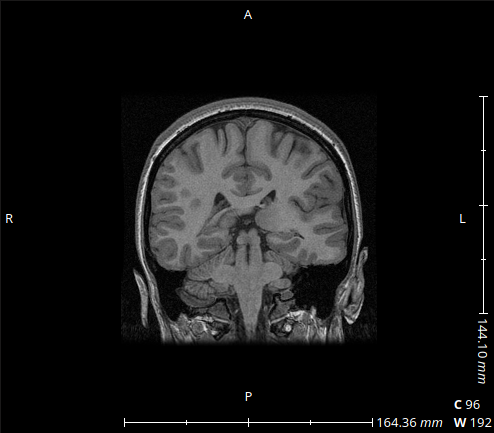
\includegraphics[width=\textwidth]{img/imageorientationindicator-002.png}
        \centering
        \label{fig:imageorientationindicator1}
    \end{figure}
    
    Każda z sześciu możliwych liter oznacza kierunek oraz zwrot w jakim jest ułożony pacjent:
    \begin{itemize}
        \item \quotett{R} - right - część prawa pacjenta
        \item \quotett{L} - left - część 
        \item \quotett{A} - anterior - przód pacjenta
        \item \quotett{P} - posterior - tył pacjenta
        \item \quotett{F} - feet - część dolna
        \item \quotett{H} - head - część górna
    \end{itemize}

    Pary poszczególnych liter tworzą osie:
    \begin{itemize}
        \item \quotett{x} - oś przechodząca od prawej do lewej strony pacjenta, \quotett{L} oznacza zwrot zgodny z osią, a \quotett{R} oznacza zwrot przeciwny, wizualizacja na rysunku \ref{fig:imageorientationindicator2}

        \begin{figure}[!htbp]
            \caption{Wizualizacja osi \quotett{x} pacjenta}
            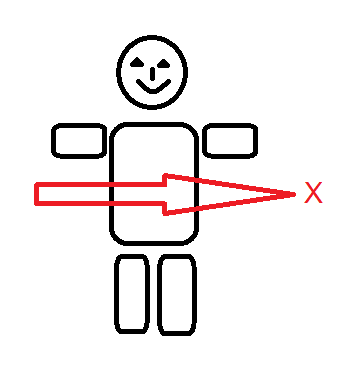
\includegraphics[]{img/imageorientationindicator-101.png}
            \centering
            \label{fig:imageorientationindicator2}
        \end{figure}

        \item \quotett{y} - oś przechodząca od przodu do tył pacjenta, \quotett{P} oznacza zwrot zgodny z osią, a \quotett{A} oznacza zwrot przeciwny, wizualizacja na rysunku \ref{fig:imageorientationindicator3}

        \begin{figure}[!htbp]
            \caption{Wizualizacja osi \quotett{y} pacjenta}
            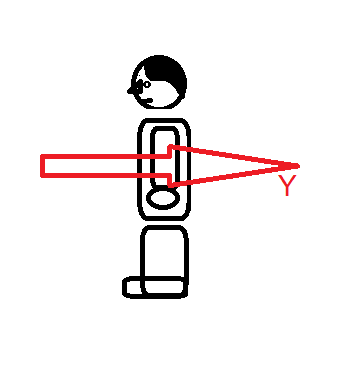
\includegraphics[]{img/imageorientationindicator-102.png}
            \centering
            \label{fig:imageorientationindicator3}
        \end{figure}

        \item \quotett{z} -  - oś przechodząca od dołu do góry pacjenta, \quotett{H} oznacza zwrot zgodny z osią, a \quotett{F} oznacza zwrot przeciwny, wizualizacja na rysunku \ref{fig:imageorientationindicator4}

        \begin{figure}[!htbp]
            \caption{Wizualizacja osi \quotett{z} pacjenta}
            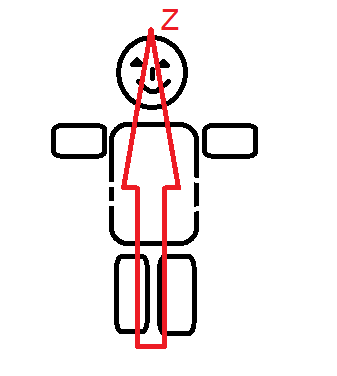
\includegraphics[]{img/imageorientationindicator-103.png}
            \centering
            \label{fig:imageorientationindicator4}
        \end{figure}

    \end{itemize}

    Informacje o orientacji oraz pozycji względem pacjenta znajdują się w odpowiednio w tagach \dicomtag{ImageOrientation}{0020}{0037} i \dicomtag{ImagePosition}{0020}{0032}.
    Wartość \dicomtag{ImageOrientation}{0020}{0037} składa się z sześciu liczb, opowiednio oznaczanych dalej X\textsubscript{x}, X\textsubscript{y}, X\textsubscript{z}, Y\textsubscript{x}, Y\textsubscript{y}, Y\textsubscript{z}.

    Standard DICOM definiuje, że te dane mają być z interpretowane w następujący sposób:    
    \[
        \begin{bmatrix}
            P_x \\ P_y \\ P_z \\ 1
        \end{bmatrix}
        =
        \begin{bmatrix}
            X_x\Delta_i & Y_x\Delta_j & 0 & S_x \\
            X_y\Delta_i & Y_y\Delta_j & 0 & S_y \\
            X_z\Delta_i & Y_z\Delta_j & 0 & S_z \\
            0 & 0 & 0 & 1
        \end{bmatrix}
        \begin{bmatrix}
            i \\ j \\ 0 \\ 1
        \end{bmatrix}
        =
        M
        \begin{bmatrix}
            i \\ j \\ 0 \\ 1
        \end{bmatrix}
    \]
    gdzie:
    \begin{conditions}
    P_{xyz} & The coordinates of the voxel (i,j) in the frame's image plane in units of mm.\\
    S_{xyz} & The three values of Image Position (Patient) (0020,0032). It is the location in mm from the origin of the RCS.\\
    X_{xyz} & The values from the row (X) direction cosine of Image Orientation (Patient) (0020,0037).\\
    Y_{xyz} & The values from the column (Y) direction cosine of Image Orientation (Patient) (0020,0037).\\
    i & Column index to the image plane. The first column is index zero.\\
    \Delta_i & Column pixel resolution of Pixel Spacing (0028,0030) in units of mm.\\
    j & Row index to the image plane. The first row index is zero.\\    
    \Delta_j & Row pixel resolution of Pixel Spacing (0028,0030) in units of mm.
    \end{conditions}

    Brak tłumaczenia jest celowy, aby uniknąć nie porozumień.

    Wyjaśnienia:
    \begin{itemize}
        \item $P_{xyz}$ oznacza punkt pozycji pacjenta wyrażony w milimetrach
        \item $S_{xyz}$ oznacza punkt pozycji pacjenta wyrażony w milimetrach w stosunku do urządzenia wykonującego pomiar, dane brane z \dicomtag{ImagePosition}{0020}{0032}
        \item $X_{xyz}$ oznacza trzy pierwsze wartości z \dicomtag{ImageOrientation}{0020}{0037}
        \item $Y_{xyz}$ oznacza trzy ostatnie wartości z \dicomtag{ImageOrientation}{0020}{0037}
        \item $i$ i $j$ oznaczają współrzędne na obrazu
        \item $\Delta_i$ i $\Delta_j$ oznaczają rzeczywistą wielkość piksela obrazu wyrażoną w mm, w algorytmie wyznaczania strony pacjenta ta wartość, może wynosić 1, ponieważ odpowiada za skale
    \end{itemize}

    Praktycznie rzecz biorąc, pierwsza macierz to wektor reprezentujący pozycje pacjenta.
    Druga jest to transformata.
    Trzecia to pozycja na obrazie.
    
    Interesuje nas wyznaczenie pozycji sześciu (punktów) na płaszczyźnie obrazu, o następujących współrzędnych, dalej używanych pod nazwą $PatientPosition$:
    \begin{itemize}
        \item \quotett{R} - $[-1, 0, 0, 1]$
        \item \quotett{L} - $[+1, 0, 0, 1]$
        \item \quotett{A} - $[0, -1, 0, 1]$
        \item \quotett{P} - $[0, +1, 0, 1]$
        \item \quotett{F} - $[0, 0, -1, 1]$
        \item \quotett{H} - $[0, 0, +1, 1]$
    \end{itemize}

    UWAGA: Wszystkie obliczenia odbywają się w współrzędnych jednorodnych.

    Wykonuje takie przekształcenie:
    \[PatientPosition = imgMatrix * ScenePosition\]
	\[imgMatrix^{-1} * PatientPosition = imgMatrix^{-1} * imgMatrix * ScenePosition\]
	\[imgMatrix^{-1} * PatientPosition = ScenePosition\]
    \[ScenePosition = imgMatrix^{-1} * PatientPosition\]
    gdzie:
    \begin{conditions}
        imgMatrix & macierz przekształcenia obrazu, o której będzie dalej\\
        ScenePosition & pozycja na obrazie, która naz interesuje \\
        PatientPosition & któryś z punktów względem pacjenta.
    \end{conditions}

    Wygląd macierzy $imgMatrix$:
    \[
        \begin{bmatrix}
            X_x & Y_x & 0 & 0 \\
            X_y & Y_y & 0 & 0 \\
            X_z & Y_z & 0 & 0\\
            0 & 0 & 0 & 1
        \end{bmatrix}
    \]
    Powyższa macierz różni się od macierzy definiowanej w standardzie.
    Po pierwsze PikselSpacing został pominięty, a konkretniej nadałem mu wartość 1.
    Po drugie pozycja z \dicomtag{ImagePosition}{0020}{0032} została zrównana do punktu zerowego, dzięki temu, wynik też będzie względem punktu zero.
    Wyznaczenie macierzy $imgMatrix$ jest jednorazowe.

    Po wyznaczeniu sześciu punktów $ScenePosition$, po jednej dla każdego punktu względem pacjenta są zapisywane. $ScenePosition$ odpowiada pozycji punktów na obrazie w pozycji startowej.

    Na scenie, której jest wyświetlany obraz, użytkownik, może obracać obraz do woli, według własnego uznania.
    Te przekształcenia, są realizowane za pomocą macierzy rotacji, dalej znana jako $rotateTransform$.
    Macierz $rotateTransform$ jest przesyłana do naszego obiektu \sokarclass{ImageOrientationIndicator} za każdym razem kiedy zostanie zmieniona.

    Ostateczne wyznaczenie pozycji punktów pacjent na obrazie odbywa sie przez przemnożenie lewostronne $rotateTransform$ i $ScenePosition$.
    \[rotateTransform * ScenePosition\]
    Wyznaczane jest w ten sposób pozycja sześciu punktów pacjenta na płaszczyźnie sceny wyświetlanej.
    Następnie określane jest na, której z ośmiu części płaszczyzny jest umieszczony dany punkt, podział płaszczyzny jest widoczny na rysunku \ref{fig:imageorientationindicator5}.
    Tej płaszczyźnie nadawany jest tytuł w postaci litery, która oznacza punkt pacjenta.
    Jeżeli punkt znajduje się w centrum, na przecięciu osi, to oznacza, że punkt znajduje się za lub przed ekranem, więc jest pomijany.
    Następnie do czterech pól wyświetlających zostają wstawione następujące teksty:
    \begin{itemize}
        \item lewe pole: tytuł części 7, tytuł części 0 i tytuł części 1
        \item górne pole: tytuł części 1, tytuł części 2 i tytuł części 3
        \item prawe pole: tytuł części 3, tytuł części 4 i tytuł części 5
        \item dolne pole: tytuł części 7, tytuł części 6 i tytuł części 5
    \end{itemize}

    Przykład:\\
    Punkt \quotett{H}, czyli punkt reprezentujący kierunek głowy, został przypisany do części 1 i odpowiednio \quotett{L} do części 7, \quotett{R} do części 3 i \quotett{F} do części 5.
    Punkty \quotett{A} i \quotett{P} zostały pominięte ponieważ znalazły się na środku.
    Do lewego pola wstawiany jest tekst \quotett{HL}, do górnego \quotett{HR}, do prawego \quotett{RF} i do dolnego \quotett{LF}.

    \begin{figure}[!htbp]
        \caption{Podział płaszczyzny sceny. Wyróżniono osiem części.}
        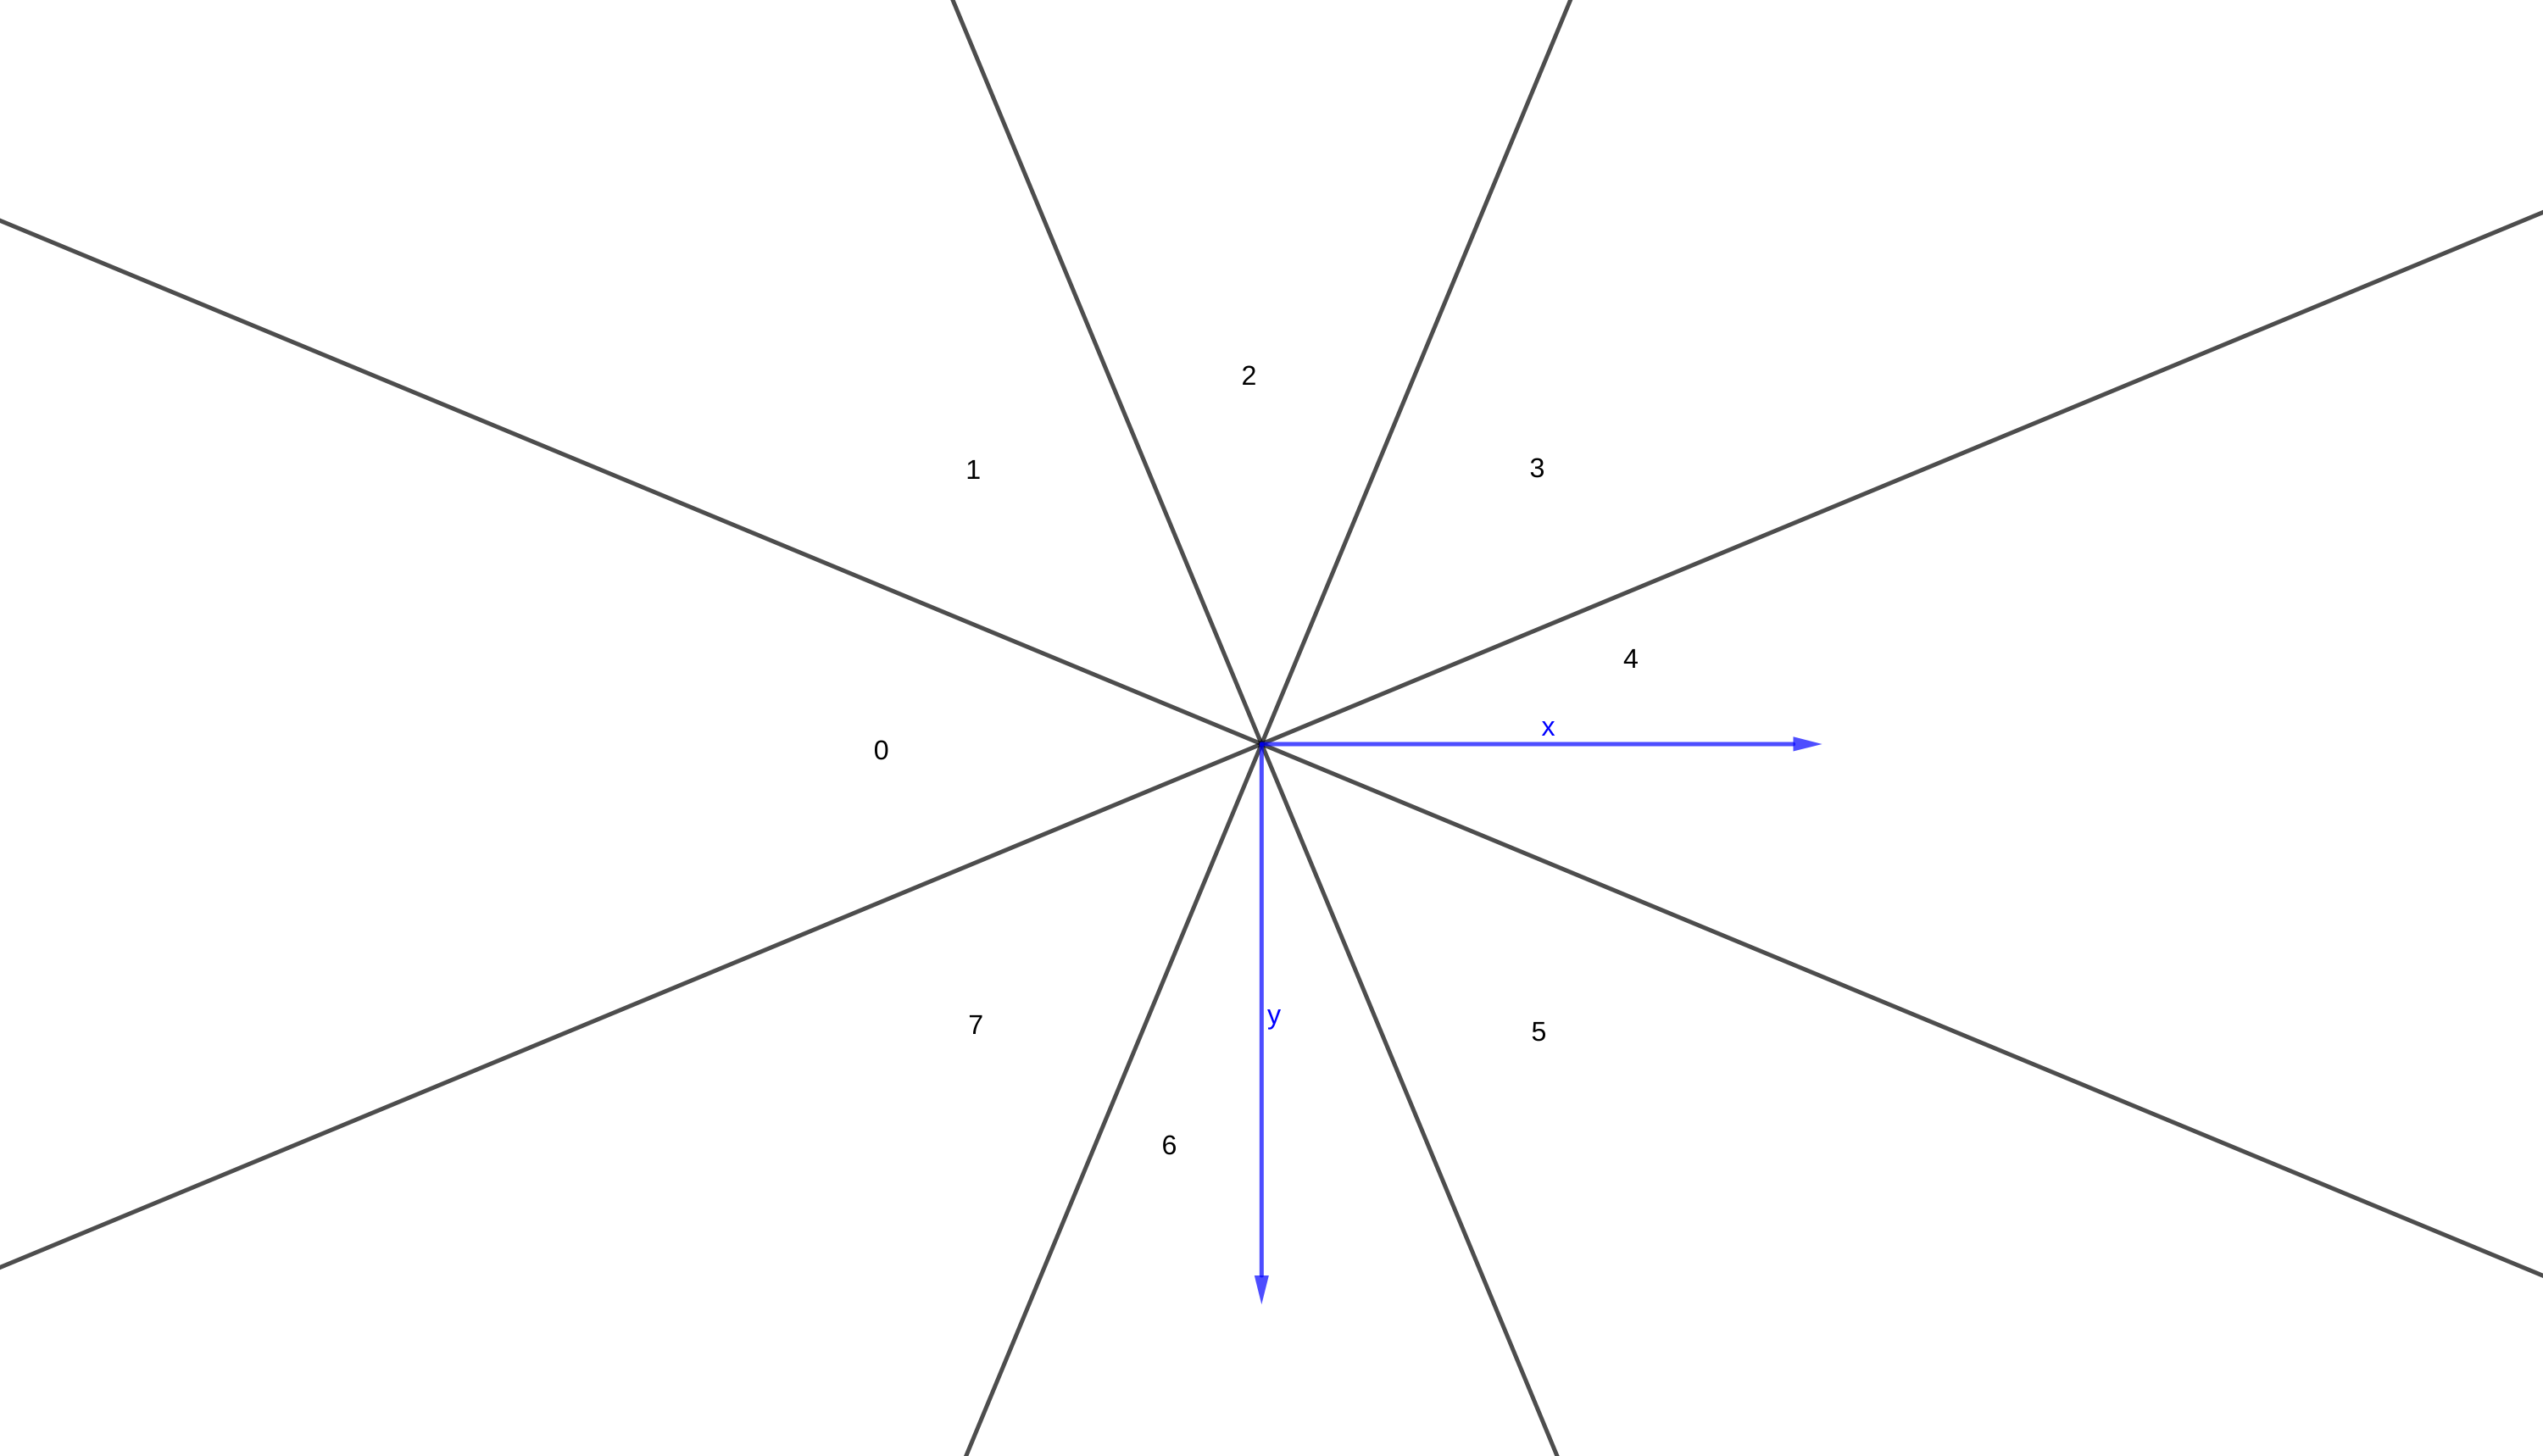
\includegraphics[width=\textwidth]{img/imageorientationindicator-300.png}
        \centering
        \label{fig:imageorientationindicator5}
    \end{figure}

    \item \sokarclass{PixelSpacingIndicator}
    
    Obiekt wyświetlający miarkę z podziałką informującą jakich rozmiarów jest obiekt na obrazie w rzeczywistości, pojawia się na dole i po prawie stronie sceny, gdy tag \dicomtag{PixelSpacing}{0028}{0030} jest obecny.
    Wygląd podziałki można zaobserwować na rysunku \ref{fig:imageorientationindicator1}.

    Podziałka dostosowuje swoją wielkość do obecnej sceny, jak i do innych elementów na scenie.
    Wartości wyświetlane biorą pod uwagę transformatę skali i rotacji obrazu.

    \item \sokarclass{ModalityIndicator}
    
    Obiekt wyświetla informacje o akwizycji obrazu.
    Dane różnią się w zależności od modalności obrazu.
    Domyślnie zawierają następujące linie:
    \begin{itemize}
        \item bla bla bla
        \item bla bla bla
        \item bla bla bla
        \item bla bla bla
    \end{itemize}

    W przypadku następujących modalności zawierają również następujące informacje:
    \begin{itemize}
        \item bla bla bla
        \item bla bla bla
        \item bla bla bla
        \item bla bla bla
    \end{itemize}
\end{itemize}


\subsection{Generowanie obrazów z danych}

Klasa \sokarclass{DicomScene} jest klasą abstrakcyjną i nie generuje obrazu, pozostawia do klasą dziedziczących po niej.

\paragraph{Cykl generowania obrazu}

Klasa \sokarclass{DicomScene} dostarcza następujące obiekty do generowania obrazu:
\begin{itemize}
    \item \cppcode{QMutex processing} mutex do zablokowania podczas generowania obrazu, aby parametry obrazu nie mogły być zmienianie podczas jego generowania.
    
    \item \cppcode{uint imgDimX} szerokość obrazu w pikselach.
    
    \item \cppcode{uint imgDimY} wysokość obrazu w pikselach.
    
    \item \cppcode{std::vector<Pixel> targetBuffer} wektor docelowego obrazu RGB o długości $imgDimX*imgDimY$.
    
    \cppcode{Pixel} to struktura reprezentujące piksel, wyglądające następująco:
    
    \cppcode{struct Pixel \{ quint8 red = 0, green = 0, blue = 0; \};}

    \item \cppcode{std::vector<char> originBuffer} wektor danych wypełniona danymi z jednej ramki o długośći iloczynu $imgDimX*imgDimY$ i ilości bajtów jednego piksela obrazu. 

    \item \cppcode{QImage qImage} obiekt obrazu.
    
    \qtclass{QImage} można zrobić z istniejącego bufora, w tym przypadku jest to \cppcode{targetBuffer}.
    Format obrazu to \qtclass{QImage::Format\_RGB888}, czyli trzy bajty, każdy na jeden kanał.

    \item \cppcode{QPixmap pixmap} obiekt obrazu do wyświetlania.
    
    Obiektów klasy \qtclass{QImage} nie da się wyświetlić, nie jest on przystosowany do wyświetlania.
    Natomiast klasa \qtclass{QPixmap} to reprezentacja obrazu dostosowana do wyświetlania ekranie, która może być używana jako urządzenie do malowania w bibliotece Qt.

    \item \cppcode{QPixmap iconPixmap} obiekt obrazu ikonu, docelowo powinien mieć 128 pikseli na 128 pikseli.
    
    \item \cppcode{QGraphicsPixmapItem *pixmapItem} wskaźnik do obiektu na scenie, który wyświetla \cppcode{pixmap}.

\end{itemize}

Generowanie obrazu jest robione przez cyzsto wirtualną funkcje \sokarfunction{DicomScene}{generatePixmap}.
Po wywołaniu funkcji obiekt \cppcode{pixmap} powinien zawierać obraz wygenerowany z obecnymi parametrami.
Funkcja zwraca również wartość logiczną, który informuje nas czy \cppcode{pixmap} rzeczywiście został zmieniony.

Całe odświeżanie obrazu jest implementowane w funkcji \sokarfunction{DicomScene}{reloadPixmap}.
Funkcja wywołuje \sokarfunction{DicomScene}{generatePixmap} i odświeża \cppcode{pixmapItem} kiedy zajdzie taka potrzeba

Generowanie poszczególnych typów obrazów jest wyjaśnione poniżej.

\subsubsection{Monochorme}

Obraz monochromatyczny to obraz w odcieniach szarości, od białego do czarnego lub od czarnego do białego. Dane są zapisane w sposób ciągły wartość po wartości.

\paragraph{Zamysł generowania obrazu}

Mamy obraz, którego piksele to n-bitowe liczby, na przykład 16 bitowa liczba całkowita.
W takiej postaci wyświetlemoe obrazu na monitorze RGB lub nawet na profesjonalnym 10-bitowym jest niemożliwe.
Należy taką liczbę przerobić na trzy liczby, reprezentujące 3 kanały RGB, czerwony, zielony i niebieski.
Dlatego do wyświetlania obrazów monochromatycznych o dużym kontraście stosuję się twór zwany okienkiem.
Jest to funkcja która mapuje n-bitwy obraz na 8-bitowy obraz w skali szarości.
8-bitów, ponieważ monitor RGB jest wstanie wyświetlić 256 odcieni szarości.

\subparagraph{Wyznaczanie okiena}
Przyjeło się, że okienko definiuje się dwoma liczbami: środkiem, oznaczanym jako $center$ i długością, oznaczaną jako $width$.
Wyznaczamy zakres okienka $x_0$ i $x_1$ z środka okienka $center$ i długości $width$.
\[x_0 = center - width / 2\]
\[x_1 = center + width / 2\]
Wyznaczamy parametry $a$ i $b$, prostej przechodzącej przez dwa punkty $(x_0, y_0)$ i $(x_1, y,_1)$.
Gdzie $y_0$ jest równe 0, a $y_1$ jest równe 255.
Funkcja okienka wygląda następująco:
\[
    f(v)=
    \begin{cases}
        0     & \text{gdy $0 \le v \wedge v \le x_0$ } \\
        a*x+b & \text{gdy $x_0 < v \wedge v < x_1$}    \\
        255   & \text{gdy $x_1 \le v \wedge v \le 1$ }
    \end{cases}
\]

gdzie $v$ to wartość piksela danych obrazu.

Następnie przepuszczamy cały obraz przez funkcje okienka i otrzymujemy obraz w skali od $0$ do $255$.
Taki odraz w skali od można już wyświetlić.
Natomiast standard DICOM przewiduje, że obraz można jeszcze wyświetlić w wielokolorowej palecie barw.
Przykład takiej palety HotIron w porównaniu do skali szarości można zobaczyć na rysunku .
Taka paleta barw nie koniecznie musi mieć 256 odcieni, dlatego lepiej jest zrobić aby okienko, mapowało na liczbę od 0 do 1, a później paleta mapowała na kolor RGB.

\begin{figure}[!htbp]
    \centering
    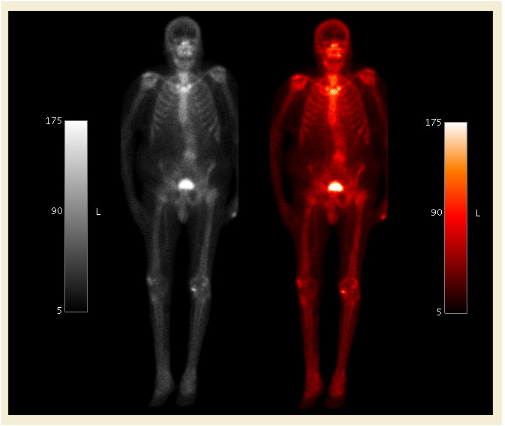
\includegraphics[width=0.7\textwidth]{img/monochrome-001.png}
    \caption{Paleta HotIron w porównaniu do palety w skali szarości}
    \label{fig:monochrome1}
\end{figure}

Teraz iterujemy po wszystkich możliwych wartościach wartośćiach obrazu i wykonujemy takie operacje.
\begin{itemize}
    \item wyznaczenie wartości okienka.
          \[y = a * x + b\]
    \item y zostaje obcięcie do 1.0 lub 0.0 jeżeli wyjdzie poza zakres od 1.0 do 0.0
    \item pobranie z palety piksel odpowiadający wartości
    \item wsadzenie piksela do tablicy, tak aby najmniejsza wartości obrazu miała indeks 0 a największy ostani
\end{itemize}


\paragraph{Implementacja algorytmu}

\subparagraph{Opis}
\par
Implementacja powyżej przedstawionego algorytmu w sposób dosłowny byłaby mało optymalna dla maszyny i wymagała by wielu pobocznych tablic oraz względnie dużej ilości mnożenia.
Trzeba też zauważyć, że do wyliczenie jakiegoś piksela nie potrzeba liczyć, żadnego innego piksela, co skutkuje, że każdy piksel można wyliczyć oddzielnie.
Dlatego najlepiej było by współbieżnie przelecieć po całym obrazie i zamienić dane na piksele.
Ale do zamiany dane na piksel, musimy mnożyć i dzielić liczby zmiennoprzecinkowe, a to do najszybszych nie należy.
Dlatego dobrym pomysłem jest zrobienie mniejszej tablicy typu LookUpTable, wypełnienie jej wszystkimi możliwymi wartościami obrazu, a następnie przerobić obraz z tablicą LUT.
Ale ponieważ tablica LUT posiada wszystkie możliwe kombinacje wartości, jej rozmiar można wyznaczyć wzorem: $2^N*3$, gdzie N to liczba bitów liczby.
Standard DICOM definiuje, że liczby mogą mieć $8$, $12$, $16$, $32$ i $64$ bity, jednakże, $12$ bitowe i tak się zapisuje w postaci 16-bitowych w pamięci RAM.
Dlatego możliwe wartości wielkości tablicy LUT to w przybliżeniu: $768$ bajtów, $196$ kilobajtów, $12,5$ gigabajtów i $56$ eksabajta($55*10^{6}$ terabajtów).
Alokowanie dwóch największych wartości może być lekko problematyczne, dlatego zrobiłem dwie implementacje algorytmu: z tablicą LUT(dla 8 i 16 bitowych obrazów i bez tablicy LUT(dla 32 i 64 bitowych obrazów).
Algorytm składa się z 3 części: wyznaczenie parametrów okna, przygotowanie okna (tylko gdy jest tablica LUT), wielowątkowa iteracja po obrazie.
\par
Okno z LUT jest implementowane przez \sokarclass{Monochrome}{WindowIntDynamic}.
Okno bez LUT jest implementowane przez \sokarclass{Monochrome}{WindowIntDynamic}.
Obie klasy dzidziczą po abstrakcyjnej klasie \sokarclass{Monochrome}{Window}m, która z kolei dziedziczy po \sokarclass{SceneIndicator}, dlatego od razu może wyświetlać obecne wartości okna.
\par
UWAGA: Standard DICOM zakłada, że danymi mogą być liczby całkowite(\cppcode{int}) oraz zmiennoprzecinkowe(\cppcode{float} lub \cppcode{double}), ale praktycznie, nie ma takich aparatów medycznych, które zapisywały by takie obrazy, gdzie dane to liczby zmiennoprzecinkowe. Dlatego założyłem, że takie obrazy nie istnieją.

\subparagraph{Wyznaczenie parametrów okna}
\par
Najpierw wyznaczam okienko, które zmienia wartości obrazu na skale od zera do jeden:
\[x_0 = center - width / 2\]
\[x_1 = center + width / 2\]
\[y_1 = 0.0\]
\[y_0 = 1.0\]
gdzie:
\begin{itemize}
    \item $center$ --- środek okienka
    \item $width$ --- szerokość okienka
    \item $x0$ i $y0$ --- współrzędne pierwszego punktu
    \item $x1$ i $y1$ --- współrzędne drugego punktu
\end{itemize}
Przeglądarka pozwala na inwersje okienka.
Dlatego kiedy użytkownik zażyczy sobie inwersji, zmienne $y0$ i $y1$ zamienią się wartoścami.

Standard DICOM przewiduje, że wszystkie dane powinny być wyskalowane, za pomocą wzoru.
\[OutputUnits = m*SV + b\]
gdzie:
\begin{itemize}
    \item $m$ --- wartość z \dicomtag{RescaleSlope}{0028}{1053}
    \item $b$ --- wartość z \dicomtag{RescaleIntercept}{0028}{1052}
    \item $SV$ --- stored values - warość pixela z pliku
    \item $OutputUnits$ --- wartość wynikowa
\end{itemize}

Wartości okienka odnoszą się do wartości już wyskalowanej, a ponieważ skalowanie całego obrazu jest czasochłonne, przeskalowaie okienka da taki sam efekt:
\[(OutputUnits - b ) / m = SV \]
więc:
\[x_0 -= rescaleIntercept\]
\[x_1 -= rescaleIntercept\]
\[x_0 /= rescaleSlope\]
\[x_1 /= rescaleSlope\]

Posiadamy, teraz dwa punkty okienka odnoszące się do wartośći obrazu.
Wyznaczam parametry prostej przechodzącej przez dwa punkty:
\[a = (y_1 - y_0) / (x_1 - x_0)\]
\[b = y_1 - a * x_1\]

\par
Teraz algorytm się rozdwaja.
Pobieranie wartości z okienka odbywa się za pomocą funkcji \sokarclass{Monochrome}{Window\zerospace::{\zerospace}getPixel()}.


\subparagraph{Implementacja dynamiczna bez tablicy LUT}

\par
W tej wersji funkcja \sokarclass{Monochrome}{Window\zerospace::{\zerospace}getPixel()}wygląda następująco:
\par
NAUCZYĆ SIĘ WSTAWIAĆ KOD C++
\par
Widzimy tutaj, że funkcja najperw sprawdza czy zakres okienka został przekroczony, następnie wylicza wartość obrazu i pobiera kolor z palety.
\par
UWAGA: ponieważ nie dysponuje rzeczywistym obrazem o pikselu danych 32-bitowym lub 64-bitowych, implementacja dynamiczna nie była testowana w warunkach rzeczywistych.

\subparagraph{Implementacja statyczna z tablicą LUT}

\subparagraph{Iterowanie po obrazie}

\paragraph{Palety}
Klasa \sokarclass{Palette} reprezentuje palety kolorów używanych do kolorowania obrazu monochromatycznego.
Paleta przerabia liczbę zmiennoprzecinkową od zera do jedynki na kolor RGB, zwracając \sokarclass{Pixel}.
Palety są wczytywane z plików XML i można definiować własne palety z poza standardem.



\subsubsection{RGB}

Obrazów zapisanych w RGB nie trzeba w żaden sposób obrabiać, dane już są prawie gotowe do wyświetlenia, należy je tylko odpowiednio posortować, tak jak wymaga biblioteka QT.
Sposób posortowania wartości w pilku określa \dicomtag{PlanarConfiguration}{0x0028}{0006}. Może o przyjąć dwie następujące wartośći:

\begin{itemize}
    \item 0 - oznacza to, że wartości pikseli są ułożone w taki sposób
        \[R1, G1, B1, R2, G2, B2, R3, G3, B3, R4, G4, B4,  ...\]
    \item 1 - oznacza to, że wartości pikseli są ułożone w taki sposób
        \[R1, R2, R3, R4, ... , G1, G2, G3, G4, ..., B1, B2, B3, B4, ...\]
\end{itemize}
gdzie:
\begin{itemize}
    \item Rn --- wartość czerwonego kanału
    \item Gn --- wartość zielonego kanału
    \item Bn --- wartość niebieskiego kanału
\end{itemize}

Wartości obrazu są przepisywane do bufora dla biblioteki QT.


\subsubsection{YBR}
Skórt YBR odpowiada skrótowi YCbCr.
Wartości są ułożone w taki sposób.
\[Y1, B1, R1, Y2, B2, R2, Y3, B3, R3, Y4, B4, R4,  ...\]

Ponieważ wartości te reprezentują kolory, są już w pewnym sensie są obrazem, ale nie można go wyświetlić, ponieważ komputery bazują na kolorach RGB.
Dlatego odpowieni algorytm konwertuje kolor YBR na kolor RGB, iterując po wszystkich wartościach obrazu.

\paragraph{Konwersja koloru YBR na kolor RGB}

YBR albo YCbCr to model przestrzeni kolorów do przechowywania obrazów i wideo.
Wykorzystuje do tego trzy typy danych: Y – składową luminancji, B lub Cb – składową różnicową chrominancji Y-B, stanowiącą różnicę między luminancją a niebieskim, oraz R lub Cr – składową chrominancji Y-R, stanowiącą różnicę między luminancją a czerwonym.
Kolor zielony jest uzyskiwany na podstawie tych trzech wartości.
YBR nie pokrywa w całości RGB, tak jak RGB nie pokrywa YBR.
Posiadają one część wspólną, co uniemożliwia wyświetlenie obrazu w stu procentach bez zniekształceń.



\section{\sokarclass{DicomSceneSet}}
\label{sec:scene-sets}

Abstrakcyjna klasa \sokarclass{DicomSceneSet} implementuje kolekcje scen.
Jest to obiekt, który grupuje w jakiś sposób sceny a następnie tworzy obiekt \sokarclass{SceneSequence}, który jest rzeczywistą sekwencją scen, ułożoną w taki sposób, jaki obrazy powinny być wyświetlane.
Są dwie implementacje zbioru scen: zbiór plików i zbiór ramek z jednego pliku

\subsection{SceneSequence}

\par
Sekwencja scen, implementowana przez \sokarclass{SceneSequence} to lista dwukierunkowa zawierającą kroki.
Implementuje strukture danych informującyh o przejściach pomiędzy scenami.
Lista ta zawiera dodatkowe informacje o obecnym stanie sekwencji:
\begin{itemize}
    \item \cppcode{int index} --- indeks w którym obecnie znajduje się sekwencja
    \item \cppcode{int direction} --- zwrot sekwencji, sekwencja może iść do przodu lub w tył
    \item \cppcode{bool sweeping} --- wartość logiczna informująca w jaki sposób ma zachować się gdy sekwencja dojdzie do końca:
    \begin{itemize}
        \item \cppcode{true} --- po dojściu do końca sekwencja skoczy do pierwszego elementu
        \item \cppcode{false} --- po dojściu do końca sekwencja zmieni zwrot
    \end{itemize}
\end{itemize}

\par
Kroki, implementowane, przez klasą \sokarclass{Step}, zawierają następujące informacje: wskaźnik do sceny oraz czas trwania sceny.


\subsection{DicomFrameSet}

\par
Obiekt tej klasy jest tworzony z jednego wczytanego pliku DICOM.
Klasa tworzy obiekt konwertera i pobiera ilość ramek w obrazie.
Tworzy jeden buffor na wszystkie ramki obrazów, a następnie dzieli go na ilość ramek.
Biblioteka GDCM nie daje dostępu do oryginalnego bufora, dlatego wymagany jest bufor pośredni.
Następnie jest tworzonych tyle obiektów scen ile ramek.
\par
Kolejność sekwencja scen jest taka sama jak kolejność ramek.
Natomiast czas wyświetlania ramki może być zapisany w różnych tagach.
To w którym tagu został zapisany informuje element o znaczniku \dicomtag{FrameIncrementPointer}{0028}{0009}, zawiera on wskaźnik do elementu o zadanym znaczniku i w zależności od znacznika.
Została zaimplementowana obsługa poniższy znaczników:
\begin{itemize}
    \item \dicomtag{FrameTime}{0018}{1063} --- element z tym znacznikiem zawiera czas trwania jednej ramki w milisekundach, każdemu krokowi jest przypisywana ta wartość trwania

    \item \dicomtag{FrameTimeVector}{0018}{1065} --- zawiera tablice z przyrostami czasu w milisekundach między n-tą ramką a poprzednią klatką. Pierwsza ramka ma zawsze przyrost czasu równy 0.
    
    \item \dicomtag{CineRate}{0018}{0040} --- zawiera ilość klatek wyświetlanych na sekunda, każdemu krokowi jest przypisywana wartość odwrotna do tej
\end{itemize}
W przypadku braku znacznika lub gdy zostaje wskazany znacznik nieznany, czas trwania ramki wynosi $83.3$ milisekundy, co odpowiada 12 klatką na sekundę.


\subsection{DicomFileSet}
\par
Obiekt tej klasy jest tworzony z wielu wczytanych plików DICOM.
Klasa nie sprawdza czy pliki odstarczone są z tej samej serii, robi to \sokarclass{DicomTabs}, opisany w sekcji \ref{sec:dicom-tabs}.
Na początku pliki są sortowane na posdtawie liczby zawartej w elemencie o znaczniku.
Dla każdego pliku jest tworzony obiekt \sokarclass{DicomFrameSet}.
\par
Sekwencja jest tworzona na połączenie sekwencji poszczególnych obrazów.


\section{\sokarclass{DicomView}}
\label{sec:sokar-dicomview}
Każda zakładka z obrazem lub obrazami jest implementowana przez klasę \sokarclass{DicomView}.

Interfejs graficzny \sokarclass{DicomView} wyświetla następujące elementy:
\begin{itemize}
    \item pasek narzędzi znajdujący się na górze - implementowany za pomocą klasy \sokarclass{DicomToolBar}, opisany w sekcji \ref{sec:sokar-dicomtoolbar}
    \item miejsce na scene z obrazem DICOM na środku - implementowany za pomocą klasy \sokarclass{DicomGraphics}, opisany w sekcji \ref{sec:sokar-dicomgraphics}
    \item suwak filmu w dolnej części - implementowany za pomocą klasy \sokarclass{MovieBar}, opisany w sekcji \ref{sec:sokar-moviebar}
    \item podgląd miniaturek obrazów w prawej części - implementowany za pomocą klasy \sokarclass{FrameChooser}, opisany w sekcji \ref{sec:sokar-framechooser}
\end{itemize}

Dodatkowo posiada obiekt \sokarclass{DicomSceneSet}, który jest zbiorem obrazów opisany w sekcji \ref{sec:sokar-scenesets}.
\sokarclass{DicomView} łączy zdarzenia wysyłane przez wszystkie obiekty.

Poniżej jest opisane zachowanie tych elementów:

\subsection{Elementy interfejsu graficznego}

\begin{figure}[!htbp]
    \centering
    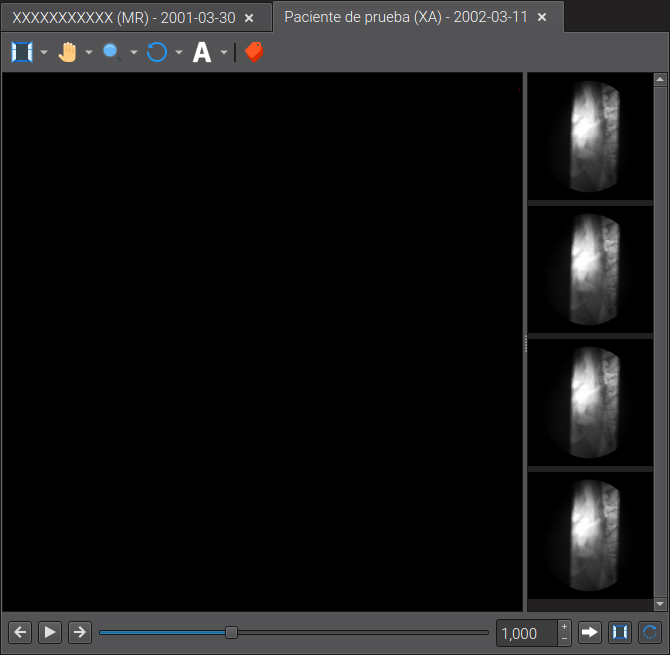
\includegraphics[width=\textwidth]{img/sokar-dicomview-001.png}
    \caption{Wygląd DicomView wraz z numeracją elementów interfejsu. Zdjęcie własne.}
    \label{fig:sokar-dicomview001}
\end{figure}

\subsubsection{\sokarclass{DicomToolBar}}
\label{sec:sokar-dicomtoolbar}
\label{sec:sokar-dicomtoolbar}
\par
Pasek narzędzi znajdujący się na górze, implementowany przez klasę \sokarclass{DicomToolBar}, dziedziczącą po klasy \qtclass{QToolBar}.
Posiada on zespół ikonek z rozwijalnymi menu kontekstowymi.

\par
Kliknięcie odpowiedniej ikony spowoduje wysłanie sygnału do obecnie wyświetlanej sceny.
Są dwa sygnały możliwe do wysłania \sokarfunction{DicomToolBar}{stateToggleSignal} lub \sokarfunction{DicomToolBar}{actionTriggerSignal}.
Pierwszy sygnał oznacza zmianę stanu paska, czyli sposób obsługi myszki, zawierał jeden argument: stan (typu \cppcode{enum}).
Sygnał ten okazał się bez użyteczny i nie jest wykorzystywany przez scene.
Drugi oznacza akcje, sygnał akcji, która powinna być wykonana na przez scenę, zawiera dwa argumenty: typ akcji (typu \cppcode{enum}) i stan akcji (typu \cppcode{bool} z domyślną wartością \cppcode{false}).

Ikony na pasku:
\begin{itemize}
    \item Okienkowanie (1)

          Stan: \cppcode{Windowing}.
          Oznacza, że horyzontalny ruch myszki powinien zmieniać szerokość okna, a wertykalny środek okna.
          Przycisk jest aktywny tylko wtedy gdy na obecna scena posiada obraz monochromatyczny.

    \item Przesuwanie (2)

          Stan: \cppcode{Pan}.
          Oznacza, że ruch myszki powinien przesuwać obraz na scenie w prawo, lewo, góra, dół, kiedy jest wciśnięty klawisz myszy.

          Rozwijalne menu zawiera tylko jedne element \enquote{Move To Center} wysyłający sygnał akcji z argumentem \cppcode{ClearPan}.

    \item Skalowanie (3)

          Stan: \cppcode{Zoom}.
          Oznacza, że ruch myszki powinien skalować obraz kiedy jest wciśnięty klawisz myszy.

          Menu rozwijalne:
          \begin{itemize}
              \item Fit To Screen --- Dopasuj do ekranu

                    Akcja: \cppcode{Fit2Screen}.

                    Po otrzymaniu sygnału obraz na scenie powinien dopasować swoją wielkość do wielkości sceny

              \item Original Resolution --- Skala jeden do jednego

                    Akcja: \cppcode{OriginalResolution}.

                    Po otrzymaniu sygnału obraz na scenie powinien dopasować swoją wielkość jeden do jedne w stosunku do piksela na ekranie.

          \end{itemize}

    \item Rotacja (4)

          Stan: \cppcode{Rotate}.
          Oznacza, że ruch myszki powinien obracać obrazem znajdującym się na scenie.

          Menu rozwijalne:
          \begin{itemize}
              \item Rotate Right --- Obróć w prawo

                    Akcja: \cppcode{RotateRight90}.

                    Po otrzymaniu sygnału obraz na scenie powinien obróć się o 90 stopni w prawo.

              \item Rotate Left --- Obróć w lewo

                    Akcja: \cppcode{RotateLeft90}.

                    Po otrzymaniu sygnału obraz na scenie powinien obróć się o 90 stopni w lewo.

              \item Flip Horizontal --- Odbij lustrzanie poziomo

                    Akcja: \cppcode{FlipHorizontal}.

                    Po otrzymaniu sygnału obraz na scenie powinien odbić się lustrzanie poziomo.

              \item Flip Vertical --- Odbij lustrzanie pionowo

                    Akcja: \cppcode{FlipVertical}.

                    Po otrzymaniu sygnału obraz na scenie powinien odbić się lustrzanie pionowo.

              \item Clear Transformation --- Wyczyść przekształcenia obrotu

                    Akcja: \cppcode{ClearRotate}.

                    Po otrzymaniu sygnału obraz na scenie powinien wyczyścić transformatę obrotu.

          \end{itemize}
    \item Informacje na obrazie (5)

          Ten element potrafi wyłączyć wyświetlanie niektórych elementów na scenie.
          Kliknięcie go odznacza lub zaznacza wszystkie pozycje w menu kontekstowym.
          Wszystkie pozycje są pozycjami odznaczanymi.

          Menu rozwijalne:
          \begin{itemize}
              \item Patient Data --- Dane pacjenta

                    Akcja: \cppcode{PatientData}.

                    Po otrzymaniu sygnału obiekt klasy \sokarclass{PatientDataIndicator} znajdujący się na scenie powinien pokazać lub ukryć się w zależności od stanu pozycji.

              \item Hospital Data --- Dane szpitala

                    Akcja: \cppcode{HospitalData}.

                    Po otrzymaniu sygnału obiekt klasy \sokarclass{HospitalDataIndicator} znajdujący się na scenie powinien pokazać lub ukryć się w zależności od stanu pozycji.
              \item Image Acquisition --- Dane akwizycji

                    Akcja: \cppcode{ModalityData}.

                    Po otrzymaniu sygnału obiekt klasy \sokarclass{ModalityIndicator} znajdujący się na scenie powinien pokazać lub ukryć się w zależności od stanu pozycji.

          \end{itemize}

    \item Tagi (5)

          Akcja: \cppcode{OpenDataSet}.

          Kliknięcie tego przycisku wyśle prośbę o otworzenie okna ze zbiorem elementów danych pliku obrazu, który jest obecnie wyświetlany na scenie.

\end{itemize}

\subsubsection{\sokarclass{DicomGraphics}}
\label{sec:sokar-dicomgraphics}

\subsubsection{\sokarclass{MovieBar}}
\label{sec:sokar-moviebar}

\par
Jest paskiem filmu w dolnej części \sokarclass{DicomView}.
Element graficzny ma dostęp do sekwencji scen i ukrywa swoją obecność przed użytkownikiem, kiedy w sekwencji jest tylko jedna scena.

\par
Pasek jest podzielony na trzy części: trzy przyciski znajdujące się po lewej, pasek pokazujący postępu sekwencji na środku i prządka z trzema przyciskami po prawej.

\par
Trzy lewe przyciski odpowiadają za poruszanie się po sekwencji.
Wciśniecie pierwszego przycisku (z indeksem 8 na rysunku \ref{fig:sokar-dicomview001}) powoduje zatrzymanie upływu sekwencji i wysłanie sygnału \sokarfunction{SceneSequence}{stepBackward} do sekwencji.
Wciśniecie drugiego przycisku (9) powoduje włączenie lub wyłączenie upływu sekwencji.
Wciśniecie trzeciego przycisku (10) powoduje zatrzymanie upływu sekwencji i wysłanie sygnału \sokarfunction{SceneSequence}{stepForward} do sekwencji.
\par
Pasek (11) pokazujący postępu sekwencji jest obiektem klasy \qtclass{QSlider}.
Odświeżanie paska jest wrażliwe na sygnał \sokarfunction{SceneSequence}{steped} of sekwencji.
\par
Elementy po prawej stronie definiuje parametry trybu filmowego.
Prządka (12), element do wprowadzania liczby zmiennoprzecinkowej klasy \qtclass{QDoubleSpinBox}.
Im większa wartość liczby tym klatki filmu są dłużej wyświetlane.
Drugi (13) przycisk pozwala zmienić sposób przemiatania.
Trzeci (14) przycisk wymusza tryb jednego okna dla wszystkich klatek filmu.
Jeżeli mamy załadowanych wile obrazów tego samego badania, to nie koniecznie muszą mieć to samo okno.
Dodatkowo ten tryb pozwala wprowadzić jednolite okienko dla wszystkich klatek po zmianie parametrów tego okienka na jednej klatce.
Czwarty (15) i ostatni przycisk służy do użycia jednej macierzy transformaty na wszystkich klatkach.

\paragraph*{Tryb filmowy}

\par
Tryb filmowy można aktywować jedynie wtedy gdy w sekwencji scen jest więcej niż jedna scena.
Włączenie trybu filmowego polega na stworzeniu obiektu klasy \sokarclass{MovieMode}.
Obiekt ten zapisuje wskaźnik go obecnie wyświetlanej sceny, to czy powinno być użyte to samo okno, oraz to czy powinna być używana ta sama transformata.
Następnie obiekt ten jest wysyłany do wszystkich scen w sekwencji.
Uruchamiany jest timer, obiekt klasy \qtclass{QTimer}, na czas równy czasu trwania sceny zapisanego w kroku przemnożonego przez liczbę z prządki.
Po upływie timera, wstawiana jest nowa scena za pomocą sygnały \sokarfunction{MovieBar}{setStep}, a timer jest ustawiany nan nowo.

\subsubsection{\sokarclass{FrameChooser}}
\label{sec:sokar-framechooser}

Ten element to wybór scen za pomocą ikon, implementowany przez klasę \sokarclass{DicomView}.
Element, podobnie jak pasek filmu ma dostęp do sekwencji scen i ukrywa swoją obecność przed użytkownikiem, kiedy w sekwencji jest tylko jedna scena.
Po wciśnięciu ikony jest zmieniana scena.

\section{\sokarclass{DicomTabs}}
\label{sec:sokar-dicomtabs}

\par
Jest to obiekt odpowiadający za wyświetlanie wielu obiektów \sokarclass{DicomView} w jednym okienku w formie zakładek.
Obsługuje również prośby o wczytanie nowych plików

\subsection{Segregacja plików DICOM}

\section{Okno główne programu}
\label{sec:sokar-window}

\par
Główne okno programu jest implementowane przez \sokarclass{MainWindow}.
Jest wywoływane od razu po uruchomieniu programu.
\par
Zawiera w sobie 4 elementy: menu, drzewo ze strukturą plików, obiekt z zakładkami \sokarclass{DicomTabs} i sugestie aby nie używać programu w celach medycznych w dolnej części okna.

\subsection{Drzewo plików i zakładki}

\par
W lewej części okna znajduje się element listy, implementowany przez \sokarclass{FileTree}, zawiera on w sobie model drzewa plików systemu, który z koleji jest implementowany przez klasę \qtclass{QFileSystemModel}.
Po wybraniu pliku, ścieżka jest przesyłana do obiektu z zakładkami.
\par
W środkowej części programu znajduje się obiekt z zakładkami, szczegółowo opisany w sekcji \ref{sec:sokar-dicomtabs}.

\subsection{Menu programu}
\label{sec:sokar-window-menu}

\par
W górnej części okna programu znajduje się menu, obiekt klasy \sokarclass{QMenuBar}.
Struktura Menu programu:
\begin{itemize}
    \item File
          \begin{itemize}
              \item Open --- otwiera okienko wyboru plików, implementowane przez \qtfunction{QFileDialog}{getOpenFileName}, następnie wczytuje plik
              \item Open Recent --- program zapisuje ostatnio wczytane pliki i może wczytać je ponownie z tego menu
              \item Export as --- zapisanie obrazu w formacie JPEG, BMP, GIF lub PNG.
                    Zapisywanie jest zaimplementowane przez funkcje \qtfunction{QImage}{save}, która umożliwia zapisanie obrazu do pliku.
              \item Exit --- wyjście z aplikacji
          \end{itemize}
    \item Help
          \begin{itemize}
              \item About Qt --- otwiera okno informacji o bibliotece Qt.
              Biblioteka Qt ma wbudowane takie okno w postaci \qtfunction{QMessageBox}{aboutQt}
              \item About GDCM --- otwiera okno z informacjami o bibliotece GDCM, implementowane przez funkcje \sokarfunction{About}{GDCM}
              \item About Sokar --- otwiera okno z informacjami o aplikacji, implementowane przez funkcje \sokarfunction{About}{Sokar}
          \end{itemize}
\end{itemize}
